%definizione generale del documento
\documentclass[a4paper,12pt,notitlepage,italian]{report}

%pacchetti importati
\usepackage[italian]{babel}
\usepackage{graphics}
\usepackage[dvips]{graphicx}
\usepackage[latin1]{inputenc}
\usepackage{verbatim}
\usepackage{makeidx}
\usepackage{fancyhdr}
\usepackage{listings}
\usepackage[monochrome]{color}
\usepackage{syntonly}
\usepackage{amsfonts}
\usepackage{amsmath}
\usepackage{amssymb}
%pacchetto di personale
\usepackage{tortorelli}

% stile di pagina(intestazione, posizione numeri...)
%\pagestyle{headings}
\pagestyle{fancy} %= interstazione piu' bella, numeri in fondo

%autore
%\author{Claudio Tortorelli}

%costruttore di indice
\makeindex

%inizio documento
\begin{document}

%elenco parole da sillabare
\hyphenation{}

%definizione del titolo
%\title{Web Testing: Teoria ed Applicazioni}

%costruttore del titolo
%\maketitle

%\begin{figure}[!h]
%\begin{center}
%	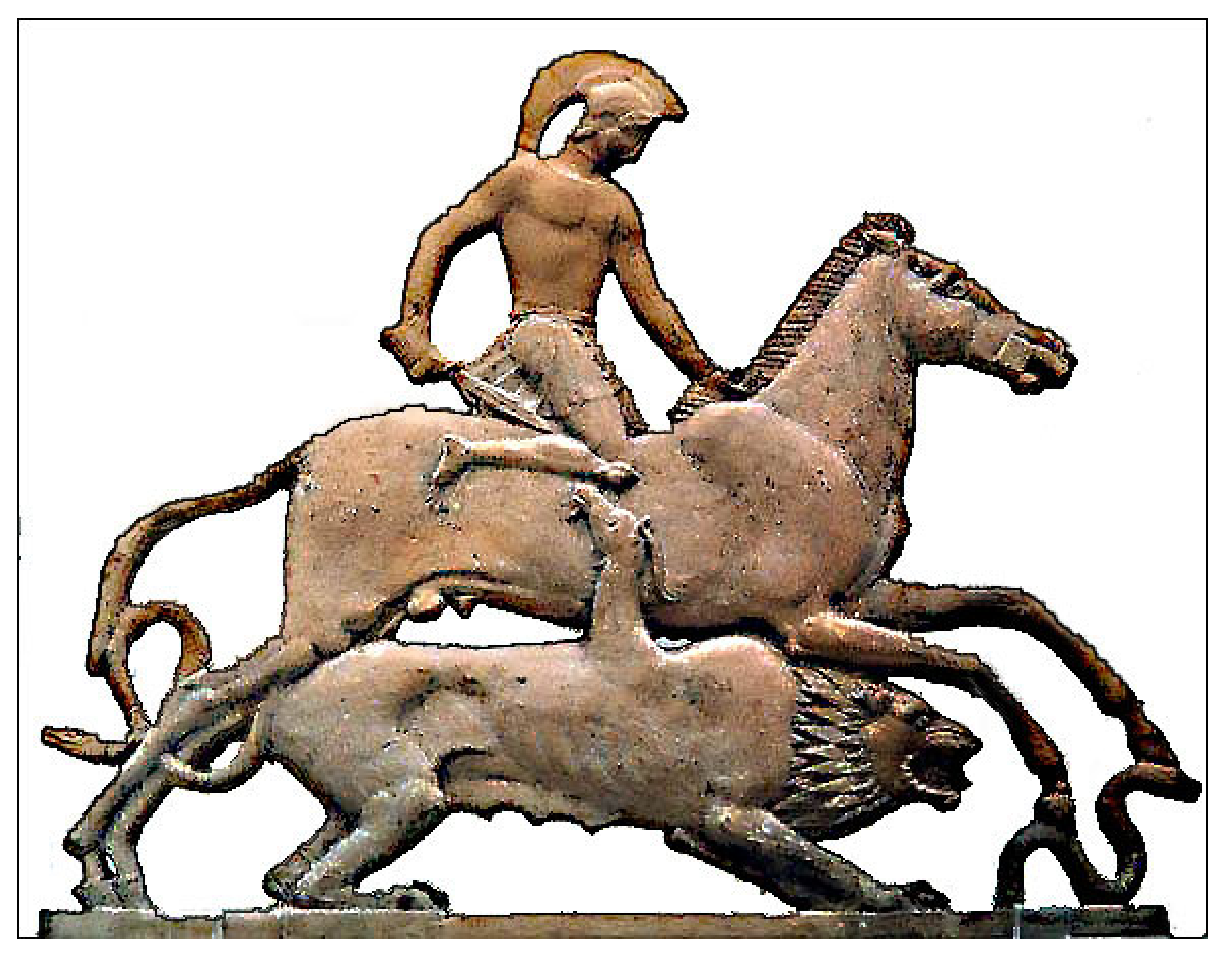
\includegraphics[width=1.00\textwidth]{immagini/bellerofonte.eps}
%\end{center}
%\end{figure}

%--- prima pagina stile tesi
\title{\vspace{-2.0cm}
\Large \bf{Universit\`a degli Studi di Firenze}\\
\large \textmd{Facolt\`a di Scienze Matematiche, Fisiche e Naturali\\Corso di Laurea
Triennale in Informatica}\\\vspace{1cm}
\Huge
\bf{Web Testing: Teoria ed Applicazioni}\vspace{1.5cm}}
\begin{figure}[!t]
\begin{center}

\includegraphics[width=.3\textwidth]{immagini/stemmaunifi2.eps}
\end{center}
\end{figure}
\vspace{1cm} \author{\bf{Laureando}: \\ Claudio Tortorelli \vspace{2cm}
\\\begin{tabular}{ccccccccc} \bf{Relatore:}&&&&&&&&\bf{Correlatore:}\\
Prof. Pierluigi Crescenzi&&&&&&&&Carlo Salinari
\end{tabular}}
\date{\vspace{2cm}29 Settembre 2003}

%costruttore del titolo
\maketitle
\thispagestyle{empty}

%numero di versione del documento
%\versione{bozza}
\newpage

%stemma universit� firenze
\thispagestyle{empty}
\begin{figure}[!h]
\begin{center}
	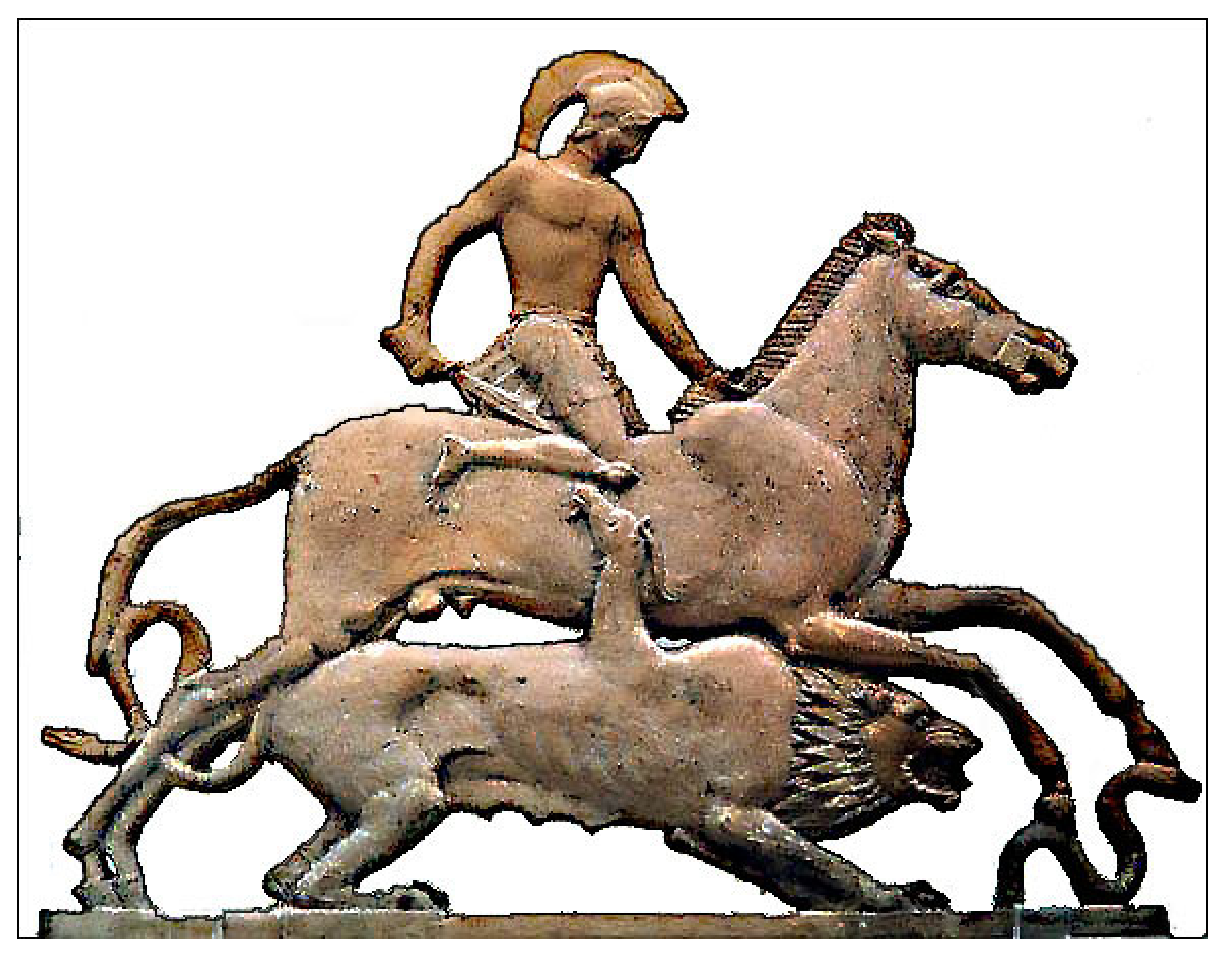
\includegraphics[width=0.7\textwidth]{immagini/bellerofonte.eps}
	\caption{Bellerofonte lotta con la Chimera}
\end{center}
\end{figure}

\newpage
%direttive di stile a fancyheader
\renewcommand{\chaptermark}[1]{\markboth{#1}{}}
\renewcommand{\sectionmark}[1]{\markright{\thesection\ #1}}
\fancyhf{} \fancyhead[LE,RO]{\bfseries\thepage}
\fancyhead[LO]{\bfseries\rightmark}
\fancyhead[RE]{\bfseries\leftmark}
\renewcommand{\headrulewidth}{0.5pt}
\addtolength{\headheight}{0.5pt}
\fancypagestyle{plain}

%posiziona l'indice costruito
\tableofcontents
\newpage

%interlinea
\linespread{1.3} %= 1.5

%----------- Inizio testo
\include{intro}
%################################################################
\part{Software e web testing}
%################################################################
\include{softwareTesting}
%----------------------------------------------------------------
\chapter{Applicazioni di rete e Web Service}
Prima di passare al web testing viene affrontata in questo capitolo una breve descrizione delle applicazioni di rete, della loro struttura e delle loro principali caratteristiche. Il software pensato per le reti, ed in particolare per il Web, � basato su paradigmi particolari che si distaccano dal contesto del software tradizionale. Conoscere queste differenze aiuta a comprendere dove e come il web testing si specializza rispetto al software testing.

\section{Il paradigma Client/Server}
Il paradigma client/server, nella maggioranza delle applicazioni di rete, definisce le modalit� di scambio delle informazioni tra soggetti distinti, permettendo di fatto la realizzazione dei servizi. 

Internet ed in generale le reti costituiscono soltanto un'infrastruttura che permette di comunicare. Allo stesso modo l'hardware di rete ed i relativi protocolli non sono altro che mezzi, i quali non prendono nessuna iniziativa nel dare inizio ad una nuova comunicazione. Sono invece le applicazioni i soggetti che, ad un alto livello di astrazione, sanno quando, come e con chi iniziare una conversazione.

Un'importante differenza tra una normale telefonata ed una comunicazione in rete � che nella seconda le applicazioni non hanno una diretta percezione della controparte. Esse devono appoggiarsi a determinati protocolli che le informino quando arriva un messaggio e da parte di chi, se � della forma attesa oppure se � stato ricevuto. I soggetti che dialogano, per evitare confusione, sono costretti ad osservare una rigida organizzazione delle informazioni scambiate, assumendo in modo coordinato un ruolo attivo o uno passivo nella conversazione.

Nel paradigma client/server questi soggetti hanno un ruolo pi� definito: l'applicazione che prende l'iniziativa del contatto viene chiamata \emph{client}\index{Client}, mentre quella che lo attende � il \emph{server}\index{Server}. Non bisogna fraintendere i significati dei termini client e server: spesso nel gergo informatico si indicano impropriamente con gli stessi nomi le macchine sulle quali tali applicazioni sono eseguite. In realt� su un singolo computer adibito a ``server'"' possono operare pi� applicazioni server contemporaneamente, per cui � consigliato associare a tali macchine dedicate il nome di ``Server-class computer'"' e ``Client-class computer'"'.
In generale un client
\begin{itemize}
	\item � un generico programma applicativo, utilizzabile per computazioni locali, che diventa client quando � richiesta una comunicazione remota;
	\item � invocato da un utente e la sua durata non coincide necessariamente con la vita del sistema nel quale risiede;	
	\item dispone di un'interfaccia utente;
	\item pu� contattare pi� server per volta.
\end{itemize}
Un server invece
\begin{itemize}
	\item � un programma specializzato nel fornire un certo servizio;
	\item pu� gestire pi� client contemporaneamente;
	\item vive durante ogni fase della vita del sistema sul quale risiede;
	\item richiede hardware e sistemi operativi appropriati;
	\item generalmente non dispone di un'interfaccia utente.
\end{itemize}
Il modello client/server impone l'asimmetria nella comunicazione, collocando le applicazioni su un piano non paritetico (al contrario  di quanto accade nel modello \emph{peer-to-peer}). La conversazione pu� svolgersi sia a senso unico sia in entrambe le direzioni. Ad ogni richiesta del client seguono una o pi� risposte del server e solo in alcuni casi il server risponde con un output continuo (ad esempio nel caso di uno stream video). 

Ma come fanno il client ed il server a scambiarsi i dati? E come riescono a contattarsi? Per risolvere simili questioni si fa affidamento sui vari protocolli che agiscono a livelli di astrazione diversi. Nell'ambito Web una delle coppie di protocolli pi� usata � \emph{TCP/IP}:\index{TCP} il primo (Transmission Control Protocol, protocollo di trasporto) permette di stabilire un canale di comunicazione tra un'applicazione ed un'altra; il secondo (Internet Protocol, protocollo di collegamento), \index{IP}ad un livello pi� basso, consente di indirizzare e spedire le informazioni. Tramite questi protocolli � possibile per il client specificare quale servizio richiedere presso un dato server e per il server rispondere in modo diretto al client richiedente. Senza scendere in maggiori dettagli si pu� schematizzare il dialogo tra client e server come segue:
\begin{enumerate}
	\item si assegna ad ogni servizio offerto un identificatore univoco;
	\item un server viene avviato e si registra presso il sistema rendendosi disponibile a soddisfare un servizio con un determinato identificatore;
	\item il server resta in attesa di chiamate;
	\item il client chiede al proprio software di protocollo quali sono gli identificatori di servizio presso una data macchina dall'indirizzo noto;
	\item ottenuto l'identificatore del servizio voluto, il client apre un canale di comunicazione con il server resosi disponibile a soddisfarlo;
	\item all'arrivo della richiesta il server sospende l'ascolto di altre chiamate (se � sincrono) e comincia ad interagire col singolo client; oppure pu� gestire concorrentemente molteplici chiamate (se � asincrono) generando altrettanti sottoprocessi;
	\item terminata la comunicazione, il server torna in attesa mentre il client chiude il canale di comunicazione precedentemente aperto.
\end{enumerate}
A seconda che la funzione computazionale sia prevalentemente a carico dell'una o dell'altra parte si parla di \emph{fat client} o \emph{fat server}\index{Fat client}\index{Fat server}. Quella dello sbilanciamento computazionale � una delle caratteristiche da valutare con maggior attenzione: attualmente, vista la notevole potenza di calcolo raggiunta dai singoli pc e l'aumento vertiginoso di connessioni ad Internet, la tendenza � quella del fat client, cos� da evitare, quando possibile, un superlavoro ai server. La funzionalit� ``lato-server'"' resta indispensabile per certe operazioni, quali, ad esempio, l'accesso a \emph{database} centralizzati. Un tipo pi� sofisticato di server � infine quello \emph{multi-livello},\index{Sever multi-livello} il quale, per soddisfare un certo servizio, � in grado di collaborare con altri server.

\section{Il Web}
Tra le varie applicazioni che hanno fatto la fortuna di Internet troviamo l'FTP (File Transfer Protocol), l'e-mail, il Network Video, Telnet, ma soprattutto il WWW (World Wide Web). Quest'ultima applicazione di rete, sviluppatasi nei primi anni '90, ha avuto un tale successo presso il grande pubblico da divenire sinonimo di Internet. La stragrande maggioranza delle applicazioni che oggi si trovano su Internet � pensata per il Web. In realt� WWW pu� essere visto come un insieme di client e server che dialogano usando il protocollo standard \emph{HTTP} (Hypertext Transfer Protocol)\index{HTTP}, il quale permette di trattare in modo uniforme quasi tutte le componenti raggiungibili tramite Internet. Le applicazioni progettate per il Web devono necessariamente comprendere questo protocollo oltre al linguaggio utilizzato per rappresentare le risorse sotto forma di ipertesto: \emph{HTML}\index{HTML} (Hypertext Markup Language). 

L'accesso al Web avviene tramite dei particolari client chiamati \emph{browser web}\index{Browser}. Essendo solitamente completi di interfaccia grafica, i browser sono relativamente semplici da usare e per questo l'accesso alle risorse di rete tramite Web � divenuto possibile anche ad utenti inesperti. I browser moderni includono anche molti \emph{plug-in}, moduli integrati capaci di rendere il browser adatto ad operazioni pi� complesse della semplice lettura di una pagina HTML: transazioni sicure, esecuzioni di \emph{script} e \emph{applet} Java, interpretazione di particolari formati multimediali sono solo alcuni esempi.

Le tipologie di server dedicate al Web sono pi� numerose, bench� spesso non altrettanto distinte: i pi� importanti sono sicuramente i \emph{web server} (contenenti le pagine HTML)\index{Web server}; poi vengono i \emph{database server} (che fungono da deposito dati) e gli \emph{application server} (che estendono i servizi offerti tramite linguaggi particolari), oltre ai pi� specifici \emph{proxy server}, \emph{search server} ed \emph{e-commerce server}.

Ogni risorsa accessibile nel Web � dotata di un \emph{URL} (Universal Resource Locator) \index{URL}univoco, al quale viene di solito associato un nome simbolico. L'associazione risorsa-URL-nome simbolico rappresenta un \emph{link}.

Il Web \index{Web}� sostanzialmente un'applicazione di Internet capace di sommare varie funzionalit� di rete e di collegare tra loro con la stessa facilit� elementi multimediali, testi, database e cos� via. Tutta una gamma di \emph{siti web}, dall'aspetto e dalle funzionalit� pi� disparate, � oggi disponibile sul Web. Bench� le applicazioni pensate per il Web non costituiscano la totalit� del software di rete, ne rappresentano sicuramente la porzione pi� ampia ed appariscente. Praticamente ogni azienda ha un proprio sito web e moltissime sono ormai quelle che sul Web fondano i propri affari (le stesse che hanno dato vita al fenomeno ``New Economy'"') fornendo particolari servizi. D'altro canto anche il software tradizionale si trova spesso a dover interagire col Web (per scaricare aggiornamenti, inviare e-mail, compilare moduli, \ldots). 

Nel capitolo 1 sono state illustrate le ragioni del software testing. Viste le problematiche intrinseche delle reti (in questa tesi non affrontate) e la variet� di aspetti inediti presenti nel software progettato per il Web, il testing diviene ancor pi� necessario.

\section{I servizi di rete}
In che consistono i famosi servizi che i server possono soddisfare? 
Nell'immaginario informatico comune una rete (nell'accezione pi� generale) � un ``deposito'"' in cui vengono messe a disposizione risorse ed informazioni di vario tipo. In Internet, la rete per eccellenza, si pu� trovare, tra le altre cose, il sito web di un comune, il servizio prenotazioni di un'agenzia di viaggi, l'e-banking di un istituto di credito, l'elenco on-line dei libri di un editore, ma anche una casella di posta elettronica o una chat. In generale, ogni volta che si raggiunge una risorsa tramite una rete, si accede ad un \emph{servizio} che essa offre.\index{Servizio di rete} Un servizio banale � quello di mostrare il contenuto di una pagina HTML; uno pi� complicato pu� essere una \emph{chiamata a procedura remota} (Remote Procedure Call). Dietro ad ogni servizio stanno uno o pi� server, una o pi� applicazioni di rete, protocolli di comunicazione adeguati e hardware dedicato.

I servizi di rete sono gi� moltissimi ma ne vengono creati sempre di nuovi per sfruttare le nuove tecnologie e far fronte alle esigenze degli utenti. Alcuni servizi sono destinati alle reti interne di aziende ed organizzazioni, altri pensati per essere accessibili da qualsiasi pc dotato di \emph{modem}. Si ha dunque un proliferare di applicazioni di rete con funzionalit�, prestazioni, struttura, finalit� e requisiti di compatibilit� molto diversi tra loro. Se da una parte questo � positivo perch� offre all'utente una maggiore libert� di scelta, dall'altra obbliga gli sviluppatori a considerare tutta una gamma di problematiche assente nel contesto del normale software centralizzato. L'interoperabilit� delle componenti, la scelta dei linguaggi di sviluppo, la coordinazione e la collaborazione delle applicazioni, i limiti stessi delle reti (raggiungibilit�, latenza e cos� via) complicano ogni fase dello sviluppo di un servizio di rete, ampliando la schiera dei possibili bug e dei relativi test da effettuare. 

In particolare � oggi molto sentito il problema delle incompatibilit� hardware e software. Da quando Internet ha permesso di collegare insieme decine di milioni di utenti, poter reperire un particolare servizio ed utilizzarlo a prescindere dalle piattaforme hardware e software � una delle principali sfide degli informatici moderni. Il testing stesso finisce per incontrare un grosso limite nelle incompatibilit� che costringono le applicazioni e le risorse di rete in un ambiente chiuso nei riguardi di piattaforme diverse. Le spese di cui si devono far carico le aziende produttrici di software per superare queste barriere e controllare poi che effettivamente siano state superate, sono molto alte. Qualcuno ha descritto metaforicamente Internet come un gigantesco \emph{arcipelago} di isole-servizi, ognuna con un proprio dialetto. Non � possibile ipotizzare in questa situazione una \emph{somma di servizi} su larga scala perch� non avrebbero capacit� di integrarsi agevolmente e vicendevolmente. Evidentemente questa non � una situazione favorevole allo sviluppo di determinati settori, come ad esempio quello dell'\emph{e-business}. Per questo le grosse industrie dell'\emph{Information Technology} si stanno accordando (e combattendo) per definire protocolli, linguaggi e piattaforme comuni.

\'E da questo sforzo che nasce il concetto di web service come estensione del servizio tradizionale.

\section{I web service}
Un \emph{web service}\index{Web service} pu� essere definito come
\emph{un'interfaccia che attraverso una rete descrive una collezione di operazioni accessibili mediante messaggistica XML.}
\index{Web service}

La caratteristica del web service rispetto al servizio web tradizionale � l'interoperabilit� e l'indipendenza dalla piattaforma su cui il servizio risiede ed � stato codificato. Una rete di grandi dimensioni � infatti tipicamente formata da infrastrutture hardware e software spesso eterogenee. Con l'uso di strumenti quali XML, SOAP, UDDI, WSDL, si scavalcano le incompatibilit�, stabilendo uno standard comune di messaggistica ad alto livello per trasferire informazioni provenienti da fonti completamente diverse. Cos� facendo si mettono in comune non soltanto i dati ma anche molte funzionalit� dei servizi, rendendole fruibili da qualunque piattaforma che ne faccia idonea richiesta. \'E una trovata non originale nel mondo dell'informatica, ma rimane fondamentalmente valida se si vuol realizzare un sistema di \emph{computazione distribuita} su grande scala (tramite Internet). Si pensi alla possibilit� di creare dei macro-servizi da combinazioni di servizi semplici sparsi nella rete. O alla facilit� con cui potrebbe essere scritta un'applicazione web se si sapesse che tutto ci� che viene ricevuto ha una codifica indipendente dalla fonte. Tutto questo si ottiene dotando il ``vecchio servizio'"' di un'efficace astrazione. Con i web service si implementa di fatto \emph{un'astrazione di servizio}, trasparente ai mezzi col quale il servizio � richiesto e svolto. 

\subsection{Architettura dei web service}
I web service possono essere visti come dei \emph{framework} di messaggi. Ad un web service � richiesto semplicemente di saper ricevere e spedire messaggi in accordo con i protocolli di rete. Nella maggior parte dei casi il loro funzionamento si riassume con uno schema classico:
\begin{itemize}
	\item il server riceve dal client un messaggio interpretabile, al quale segue l'avvio di una o pi� applicazioni in remoto;
	\item terminata l'elaborazione viene inviato in risposta al client un messaggio con il risultato.
\end{itemize}
La novit� sta nell'utilizzo di meccanismi standardizzati di impacchettamento dei dati, abbinati ad XML (eXtensible Markup Language),\index{XML} un linguaggio di codifica delle informazioni universalmente riconosciuto e sempre pi� utilizzato. 

A livello logico un web service pu� essere scomposto in due componenti principali:
\begin{itemize}
	\item un \emph{service listener}, in grado di comprendere i protocolli di trasporto ed impacchettamento. Esso rimane in attesa di messaggi in arrivo;
	\item un \emph{service proxy} in grado di tradurre le richieste in effettive chiamate all'applicazione retrostante. 
\end{itemize}
Un'altra caratteristica dei web service � l'\emph{integrazione dinamica}\index{Integrazione dinamica} con la piattaforma sulla quale risiede l'applicazione server. Si vuole infatti garantire l'indipendenza da tale piattaforma ed al tempo stesso fornire un meccanismo che permetta di orientarsi nella ricerca di un servizio, con la libert� di variare i parametri dei servizi offerti. Questa configurazione ``sul momento'"' � realizzata nella \emph{web service architecture} da vari soggetti: \index{Web service architecture}
\begin{enumerate}
	\item un \emph{service provider} pubblica un elenco dei servizi che pu� offrire in un certo momento;
	\item questo elenco � reso noto ad un \emph{service registry} (fase di pubblicazione del servizio);
	\item un \emph{service requestor} o \emph{consumer} (essere umano o altra applicazione web) si rivolge al service registry per trovare un servizio a lui utile e questo gli riporta l'indirizzo del service provider in grado di fornirglielo;
	\item ottenuto tale indirizzo il service requestor tenta di accedere al servizio vero e proprio presso il service provider (fase di \emph{bind});
	\item conclusa positivamente la fase di bind lo scambio dei dati avviene direttamente tra il service requestor ed il service provider.
\end{enumerate}
Questa architettura permette di variare il numero, il tipo e l'indirizzo di certi servizi offerti anche a run-time, dinamicamente e senza coinvolgere necessariamente chi richiede il servizio.

%\begin{figure}[h]
%	\begin{center}		%\includegraphics[width=1.00\textwidth]{D:/Documenti/TeX/tesi/immagini/schemaSe2.eps}
%	\end{center}
%	\caption{Schema di architettura dei web services}
%	\label{fig:schemaSe}
%\end{figure}
	
Alternativo e complementare al modello di architettura analizzato c'� il \emph{modello Peer},\index{Modello Peer} che ha una configurazione pi� flessibile in quanto la distinzione tra service provider, registry e consumer non � rigida. Ogni peer (punto o nodo) della rete pu� costituire un'entit� ``polimorfa'"' che assume a seconda delle necessit�, dei servizi richiesti e del soggetto che li richiede, uno dei ruoli necessari alla realizzazione del servizio. 

\section{Conclusioni}
In questo capitolo � stata data una veloce descrizione dei meccanismi che stanno dietro al software a cui si applicheranno le tecniche di web testing illustrate nel prossimo capitolo. Chi effettua web testing � per� tenuto ad approfondire nei dettagli la propria conoscenza delle reti, delle loro qualit� e problematiche. \'E fondamentale aver presenti i limiti delle applicazioni web e le loro diversit� rispetto al software tradizionale perch� sottovalutare o ignorare queste differenze pu� portare a test formalmente corretti ed efficaci nella teoria ma insufficienti nella realt�. 
%----------------------------------------------------------------
\chapter{Il web testing}
In questo capitolo saranno analizzati in modo pi� dettagliato i punti critici delle applicazioni web e di conseguenza dove si rende necessario il web testing. Non verranno proposti dei test specifici ma ci si limiter� ad evidenziare il loro obiettivo finale. Questo perch� ogni team di sviluppo o di verifica ha a disposizione vari strumenti e, per effettuare test concreti, pu� combinarli con altrettante metodologie. Salendo invece ad un livello appena superiore � conveniente focalizzare l'attenzione sugli obiettivi del web testing, in particolare su come scomporre qualitativamente in categorie questa attivit� al fine di raggiungere pi� facilmente gli scopi preposti.

\section{Cosa si deve testare}
Dal software testing deriva (storicamente e metodologicamente) il web testing, per cui la maggior parte delle conoscenze accumulate per il primo � stata utile per il secondo. La diversit� di contesto tra i due tipi di testing implica per� differenti modalit� di applicazione e valutazione. La verifica dei link, ad esempio, � un'operazione che non viene effettuata di norma per il software tradizionale. In ogni caso,  anche quando gli aspetti da testare sono presenti sia nel web che nel software testing, � difficile che la semantica rimanga la stessa: uno script pu� essere visto come un metodo di un oggetto, ma quando si testa nel suo contesto molte somiglianze spariscono. 

Un software che lavora localmente non viene spesso a contatto con problematiche quali lunghi tempi di download, latenze di rete, traffico ed indirizzamento delle informazioni, utilizzo condiviso da parte di vari utenti (anche numerosi). Altri aspetti come la sicurezza o l'autenticazione degli utenti hanno poi un peso minore. Persino l'interfaccia grafica, che per un software tradizionale � definita una volta per tutte in fase di sviluppo, nelle applicazioni di rete pu� essere soggetta ad interpretazioni diverse da parte dei browser che la visualizzano.

Le caratteristiche tecniche non sono d'altra parte le uniche a fare la differenza. Nel momento in cui un sito web viene messo in rete, lo si espone all'utilizzo di un'utenza composita e variegata, di cultura, conoscenze informatiche ed interessi anche molto diversi.
Questo avviene indipendentemente dalle reali intenzioni ed ambizioni  degli sviluppatori. In altre parole l'usabilit�, gi� fattore critico nel software testing, � ancora pi� importante nelle applicazioni web che interagiscono direttamente con utenti spesso non definiti in fase di progetto. 

Per rimarcare ulteriormente quanto il differente contesto influisca sui test destinati ad un'applicazione web, si ricordi che quasi tutte queste applicazioni hanno la necessit� di un aggiornamento continuo (a volte automatico) dei propri contenuti o della propria interfaccia. Quindi, mentre nel software ``statico'"' tutto (a parte il valore dei dati da immettere) � definito in fase di sviluppo, nelle applicazioni web si ha molta pi� ``dinamicit�'"', a volte in funzione dell'utente stesso. Tutto questo fa sorgere numerosi problemi di coerenza, rendendo necessari altrettanti test.

La qualit� di un'applicazione web pu� dipendere da un dato insieme di aspetti, tra cui:
\begin{itemize}
	\item le interfacce utente;
	\item le funzionalit�;
	\item l'accesso ai database;
	\item la facilit� e la correttezza del processo di installazione/disinstallazione;
	\item la facilit� di configurazione e la compatibilit�;
	\item la sicurezza e l'autenticazione;
	\item le performance (con l'esecuzione in stato di stress).
\end{itemize}
Si noti che ognuno degli aspetti elencati (che non saranno necessariamente tutti presenti) � facilmente riscontrabile dagli utenti, dagli operatori o dall'amministratore. Per questo un bug che interessi una di queste caratteristiche pu� incidere notevolmente sull'affidabilit� e l'usabilit� dell'applicazione. 

Oltre ai test riguardanti le peculiarit� evidenziate, in fase di sviluppo rimangono da verificare alcune qualit� specifiche meno appariscenti: l'architettura dell'applicazione, le modalit� di dialogo tra le componenti, l'efficienza degli algoritmi ed in generale tutto quello che si addice ad un testing white box.

\section{Una panoramica generale}
I \emph{test types}\index{Test types} sono categorie di test pensate per catalogare determinate classi di errori.  La suddivisione dei test in tipologie consente di individuare pi� agevolmente le aree logiche del software ed i test destinati a verificarle in determinate fasi dello sviluppo. I test sottoelencati sono comuni sia al software che al web test. Nella prossima sezione saranno riprese in esame dal pi� specifico punto di vista del Web.

\subsection{Acceptance testing}
\begin{itemize}
	\item \emph{Development acceptance test}: consiste in una serie di test effettuati in fase di sviluppo con l'obiettivo di assicurare un livello minimo di qualit�. A sua volta si suddivide in 	
\begin{enumerate}
	\item \emph{Release acceptance test (RAT)}: test effettuato per ogni \emph{release} per verificare che sia sufficientemente stabile prima di effettuare ulteriori test. Normalmente consiste in controlli sui valori di input e di output.
	\item \emph{Functional acceptance simple test (FAST)}: � il primo test funzionale effettuato su ogni release in fase di sviluppo, volto a controllare la presenza delle caratteristiche chiave nell'applicazione. Superare anche questo tipo di test � una condizione necessaria per poter successivamente applicare test pi� complessi.
\end{enumerate}

\item \emph{Deployment acceptance test}: prevede l'installazione e la configurazione dell'applicazione in quello che sar� il reale ambiente di lavoro (o una sua versione approssimata). Spesso infatti, fino ad un certo grado di sviluppo, il software viene testato in ambienti di lavoro estranei a quello di destinazione. Collocare il programma nel contesto giusto � essenziale prima di procedere con test di livello superiore.
\end{itemize}

\subsection{Feature-level testing}
Accertata una correttezza di base del software si procede col verificare, stavolta in modo approfondito, le sue caratteristiche:
\begin{itemize}
	\item \emph{Task-oriented functional test (TOFT)}: i TOFT consistono in un'analisi positiva dei compiti che l'applicazione dovrebbe saper svolgere, sulla base di quanto stabilito nei documenti di analisi e progetto.
	\item \emph{Forced-error test (FET)}: a differenza dei TOFT, i FET agiscono negativamente, costringendo l'applicazione a lavorare in condizioni di errore. Si sfruttano questi test per generare contemporaneamente una lista di errori possibili e verificare come il programma li gestisce.
	\item \emph{Boundary test}: controllano come il programma risponde nei casi in cui l'input assume valori estremi o critici. 
	\item \emph{System-level test}: sotto questo nome vanno tutti i test volti a verificare come l'applicazione interagisce col sistema sottostante.
	\item \emph{Real-world user-level test}: vengono eseguite le operazioni che si suppone siano pi� frequenti da parte degli utenti.
	\item \emph{Load/Volume test}: questi test riguardano lo studio di come il programma gestisce grandi quantit� di dati e computazioni eccessive (non necessariamente estreme).
	\item \emph{Stress test}: in questo caso si forza il software a lavorare in condizioni di risorse limitate (memoria, spazio su disco, larghezza di banda sulla rete e cos� via). L'obiettivo � individuare il limite oltre il quale le funzionalit� non sono pi� garantite.
	\item \emph{Performance test}: l'obiettivo di questi test � scoprire la strategia giusta per mantenere le funzionalit� del programma sopra un certo livello di efficienza nella maggior parte dei casi.
	\item \emph{Regression test}: sono test usati per confermare che i vecchi bug siano stati corretti adeguatamente, senza danneggiare altre funzionalit�. Sono di solito ripetuti ad intervalli predefiniti.
	\item \emph{Compatibility and configuration test}: in questi test si vanno a controllare le funzionalit� del software nei riguardi di particolari componenti esterne (periferiche, sistemi operativi, \ldots). Una strategia spesso adottata � quella che prevede l'esecuzione di un sottoinsieme di FAST o TOFT in vari ambienti di lavoro.
	\item \emph{Documentation/On-line help test}: anche come il programma viene in aiuto dell'utente � un aspetto da testare. Viene controllata dunque l'accuratezza della documentazione, insieme all'usabilit� ed alla funzionalit� degli help in linea.
	\item \emph{Install/Uninstall test}: testare che l'installer metta l'applicazione in condizioni di funzionare correttamente e l'uninstaller la rimuova dal sistema, � una questione di ``bon-ton'"' informatico. L'utente non deve preoccuparsi di questi ``dettagli'"' pi� di tanto: esso � interessato solo all'uso del software. Per le applicazioni web si pu� avere un'installazione/disinstallazione dal lato client, dal lato server o da entrambi i lati.
	\item \emph{User interface test}: la facilit�  d'uso dell'interfaccia utente � un altro punto da testare. Con questi test si mettono alla prova l'usabilit�, l'aspetto grafico, la navigabilit�, l'accessibilit� ed il \emph{feedback} dato dell'interfaccia.
	\item \emph{Security test}: per molte applicazioni la sicurezza � un aspetto cruciale. Con questi test si valuta se la politica adottata per rendere il software sicuro � sufficiente rispetto al livello di protezione richiesto.
	\item \emph{Unit test}: rientrano in questa categoria di test tutti quelli volti a valutare la correttezza delle singole unit di codice prima che vengano integrate nel software. \'E un tipo di testing effettuato ``in privato'"' dai singoli programmatori.
\end{itemize}
 
\section{Analisi di alcune categorie di web testing}

Segue ora la presentazione di alcune tra le principali classi di web testing attraverso le problematiche specifiche delle applicazioni web.  In particolare verranno trattate quelle che pi� direttamente interessano il tool di web testing realizzato per la tesi (Bellerofonte) e l'applicazione web alla quale sar� applicato (Orbilio). 
Per maggiori dettagli si rimanda ai riferimenti bibliografici \cite{2.2}.

\subsection{User Interface test}
Testare un'interfaccia vuol dire verificare disegno ed implementazione delle sue componenti. Il testing delle UI (User Interface) � condotto sia con test appositi sia nel corso di altri test (ad esempio i TOFT o i test di usabilit�).
\begin{itemize}
	\item Per quanto riguarda il \textbf{disegno di interfacce}, le migliori valutazioni provengono dagli utenti finali. Naturalmente esistono anche delle autorevoli linee guida da seguire, basate su euristiche e considerazioni derivate dalla psicologia cognitiva. \'E per� sempre utile coinvolgere campioni di utenza per avere impressioni dirette sull'usabilit�, la navigabilit�, la chiarezza e l'accessibilit� dell'UI. Una buona interfaccia deve in sostanza supportare l'utente in ogni possibile interazione con l'applicazione, ma deve farlo senza che l'utente si debba mai porre troppe domande.

\'E essenziale rispondere subito a due interrogativi: 
\begin{itemize}
	\item ``Chi saranno gli utenti dell'applicazione?'"'. Anzitutto � necessario sapere se gli utenti dell'applicazione web si troveranno dal lato server o da quello client. Ai primi si attribuisce in genere una funzione amministrativa e dunque si suppone che il loro livello tecnico sia sufficientemente alto. Altrettanto non si pu� ipotizzare per gli utenti client-side: essi accederanno all'applicazione prevalentemente tramite un browser per usufruire del servizio offerto, ma spesso senza disporre di conoscenze specifiche. In questo caso l'interfaccia assume un ruolo-guida molto pi� rilevante.
	
Per classificare l'utenza inoltre si ricorre ad un insieme di parametri qualitativi: esperienza informatica, esperienza del Web, conoscenza del campo applicativo del software ed esperienza nell'uso di applicazioni simili.

	\item ``Quale approccio generale seguire nel disegno?'"'. Individuata l'utenza tipica, bisogna pensare a quale schema generale di disegno sia pi� adatto. Ad esempio, per supportare utenti ``inesperti'"' si pu� considerare l'inserimento di numerose schermate di \emph{wizard}, che guidino passo dopo passo attraverso scelte complicate. Importante � poi la \emph{metafora}\index{Metafora} che deve accomunare ogni elemento del disegno: una metafora � un ponte tra le esperienze dell'utente nel mondo reale (ed informatico) e quelle fatte nell'applicazione. Ad esempio si pu� scegliere di rappresentare graficamente una funzione ``calcolatrice'"' in tanti modi diversi, ma disegnarla simile alle calcolatrici reali aiuta sicuramente l'utente a capirne l'uso. Una metafora sbagliata disorienta notevolmente un utente.
\end{itemize}
	
Un programmatore non pu� prevedere tutte le singole impressioni che la sua interfaccia susciter� negli utenti, ma pu� verificare oggettivamente che il significato di un elemento sia consistente ogni volta che appare nell'interfaccia. Gli errori stessi dovrebbero essere presentati in modo coerente al resto del disegno.

Il disegno di un'interfaccia web non si limita ad interessare la ``piacevolezza'"' dell'utilizzo, riguarda da vicino anche l'interazione in termini di input/output. Durante l'uso dell'applicazione, l'utente dovr� inserire spesso dei valori in input per poi attendersi la presentazione dei relativi output. In queste fasi l'applicazione lo dovr� guidare ed aiutare tramite tutta una serie ben combinata di \emph{controlli grafici}: dai semplici \emph{tag} HTML (form, bottoni, \ldots) ai controlli dinamici realizzati in Java, ActiveX, JavaScript e cos� via, fino all'utilizzo di \emph{Server-Side Includes} (SSI) e \emph{Cascading Style Sheets} (CSS). La presentazione degli output � vitale quando si ha a che fare con dati provenienti da database in quanto occorre saperli organizzare in tabelle che ne permettano una facile e veloce consultazione. 

\item L'\textbf{implementazione dell'interfaccia} ha invece un occhio di riguardo per le operazioni che stanno dietro ogni elemento. In sostanza si richiede ad ogni componente di ``fare quello che ci si immagina che faccia a giudicare dal disegno'"'. I test di questo tipo sono spesso svolti in concomitanza di quelli funzionali. Alcune complicazioni specifiche del Web circa l'implementazione di interfacce sono: 
\begin{itemize}
	\item la diversa interpretazione da parte dei vari browser;
	\item l'invio ritardato al server degli input immessi dall'utente: fin quando l'utente non d� esplicito avvio alla trasmissione, i valori immessi sono presenti solo sul client e quindi c'� pericolo di perdita dei dati, bench� l'interfaccia dia l'impressione che ogni inserimento sia definitivo;
	\item l'esecuzione di script non � sempre consentita sul client;
	\item il bottone ``Back'"', presente in ogni browser, complica le relazioni tra le pagine web, in quanto, consentendo di tornare all'ultima pagina visitata, pu� non rispettare i link presenti sulla pagina attuale;
	\item la risoluzione di schermo ed i caratteri installati nel sistema influiscono sulla presentazione dell'interfaccia.
\end{itemize}
\end{itemize}

\subsection{Functional test}
Il testing delle funzionalit� di un'applicazione web riguarda la verifica di ci� che l'applicazione dovrebbe fare, relativamente alle aspettative dell'utente. In questa categoria rientrano molte sotto-tipologie di test: i FAST, i TOFT, i boundary test, i forced-error test e parte dei security test.

\begin{itemize}
	\item FAST: come descritto nella sezione precedente, i FAST mirano a
dimostrare la correttezza delle funzionalit� ad un basso livello, senza prendere in considerazione le combinazioni con altre funzionalit� (testate nei TOFT). Nel caso delle applicazioni web, uno dei loro obiettivi � verificare il comportamento dei singoli componenti dell'interfaccia (text-box, bottoni, bandierine, ma anche i link grafici e testuali), i loro eventuali valori di default e via dicendo.	Sono considerate caratteristiche chiave in ambito Web anche operazioni come il log in/log out, la ricerca, l'autenticazione ed il recupero password smarrite.

\item TOFT: nei TOFT si pone l'attenzione sulla capacit� dell'applicazione di soddisfare compiti pi� articolati, esplicitamente richiesti nel progetto. In generale vengono eseguiti dopo i FAST, in quanto si basano su liste di caratteristiche di base prese gi� singolarmente in esame. \'E da stabilire in questo contesto se combinazioni opportune di queste caratteristiche riescono a soddisfare dei requisiti particolari. Ad esempio potrebbe essere richiesto che il task composto dalla sequenza log in e autenticazione venga eseguito entro un dato tempo.
	\item Forced-error test: lo scopo di questi test � trovare le condizioni di errore ignorate o gestite male. Ad esempio, se un campo di un modulo ammette come valide solo sequenze di caratteri alfabetici, l'introduzione di un numero genera una condizione di errore che deve essere gestita correttamente affinch� il test sia considerato superato. Per ogni condizione di validit� ce n'� sempre una di invalidit�. La maggiore complicazione nell'ambito Web consiste nella quantit� di soggetti che entrano in gioco per alcune transazioni: oltre al client ed al server vi � tutta una catena di ``intermediari'"' (tra cui la rete stessa) che concorrono alla realizzazione di un certo servizio, ognuno dei quali pu� generare errori difficilmente prevedibili (e gestibili) nel complesso.	
	\item Boundary test: i boundary test considerano i limiti nel dominio di ogni funzionalit� e la mettono alla prova per tali valori. Possono considerarsi delle estensioni dei forced-error test e dei TOFT.	
\end{itemize}

Una sottotipologia che riassume un p� tutte quelle elencate � quella degli \emph{Exploratory test}, che consiste nello ``spostarsi'"' all'interno dell'applicazione e testare di volta in volta le funzionalit� incontrate.

\subsection{Database test}
Tutte le applicazioni web che necessitano di accesso ai dati hanno bisogno di un \emph{database server}\index{Database server}. I database giocano un ruolo importantissimo nel Web. Essi ospitano i dati delle applicazioni e gestiscono le loro operazioni di inserimento, cancellazione ed interrogazione. Una delle tecnologie comunemente usate per i web-database � quella dei \emph{database relazionali}\index{Database relazionali}. I database relazionali sono composti da tabelle che possono essere facilmente riorganizzate e visitate. I dati sono contenuti in \emph{record} relativi a dei campi a loro volta appartenenti alle tabelle. In ambito Web poi, l'archivio � spesso disperso tra molteplici server, per questo si parla di \emph{database distribuito}\index{Database distribuito}. Il database server viene normalmente implementato tramite un apposito linguaggio, \emph{SQL} (Structured Query Language), che offre tutta una serie di primitive per manipolare i dati nelle tabelle bidimensionali. 

Anche nel caso dei database vi sono molti punti di interazione tra l'applicazione client, quella server, il database server e gli altri soggetti della catena. Perci� � necessario applicare procedure di testing a vari livelli. Particolarmente delicata � la funzione degli script che gestiscono i dati, poich� rappresentano un'astrazione del database per le applicazioni client e server. 

Due classi di problemi derivate dai bug nei database sono gli \emph{integrity error} e gli \emph{output error}\index{Integrity error}\index{Output error}. Gli integrity error possono essere visti come un danneggiamento o una perdita dei dati contenuti nei record; gli output error invece si hanno quando, nonostante i dati siano correttamente archiviati, non � possibile recuperarli. I sintomi evidenziati da entrambe le classi di bug sono simili, per questo � difficile capire di che tipo di errore si tratta (e dove � localizzato) con i test black-box. Vi sono invece numerosi tipi di test white-box che permettono l'individuazione di bug nei database con discreta efficienza. I test black-box rimangono comunque indicati per rilevare le anomalie, in quanto vengono eseguiti dal browser e dunque rispecchiano direttamente il comportamento del database dal punto di vista dell'utente. 

\subsection{Installation test}
Questo tipo di test si concentra prevalentemente sull'eliminazione di tutta una serie di problemi che possono sorgere in fase di installazione dell'applicazione web: 
\begin{itemize}
	\item variabili di sistema non trovate implicano un'auto-configurazione scorretta;
	\item copie incomplete di file dovute a errori di trasmissione;
	\item incompatibilit� hardware/software;
	\item interferenze da parte dell'utente in momenti critici;
	\item interferenze da parte di \emph{firewall} ed antivirus.
\end{itemize}
La maggior parte delle applicazioni web prevede un'installazione solo dal lato server, ma ci sono anche casi in cui, viste le particolari funzionalit� da svolgere, i comuni browser sono ritenuti non idonei e viene realizzato un apposito client. In queste eventualit� i test devono riguardare anche il lato client dell'applicazione. 

Testare i processi di installazione presuppone una solida conoscenza dei sistemi operativi e dell'ambiente in cui il tool di installazione operer�. Alcune delle principali operazioni svolte dal software di installazione (\emph{installer}) sono:
\begin{itemize}
	\item lanciare l'installazione dall'host sorgente;
	\item mantenere un log di installazione nell'host destinazione;
	\item recuperare le informazioni necessarie sull'ambiente destinazione ed installare l'applicazione secondo le opzioni scelte dall'utente;
	\item decomprimere eventuali file compressi;
	\item aggiornare il registro di sistema (Windows).	
\end{itemize}
A queste operazioni � associato un insieme di possibili errori suddivisi in classi:
\begin{itemize}
	\item \emph{Functionality error}: quando l'installer fallisce il proprio obiettivo di completare l'installazione per i motivi pi� svariati (impossibilit� di effettuare il \emph{reboot}, mancanza di spazio su disco, impossibilit� di creare directory e cos� via);
	\item \emph{User interface design error}: quando l'interfaccia utente non rappresenta correttamente i risultati dell'installazione;
	\item \emph{User interface implementation error}: quando l'interfaccia non implementa bene alcune funzionalit�, quali ad esempio la semantica delle opzioni di setup propedeutiche all'installazione;
	\item \emph{Misinterpreting collected information}: quando le informazioni raccolte sul sistema non sono quelle reali;
	\item \emph{Operating system error}: quando avviene un errore del sistema operativo sottostante all'applicazione, durante l'installazione.	
\end{itemize}
Terminata con successo l'installazione � comunque indicato verificare, con test black-box, che effettivamente tutto sia andato a buon fine.

D'altro canto, se si vuol offrire un servizio completo, � necessaria anche la presenza dei tool che si occupano della disinstallazione dell'applicazione (salvando eventualmente i dati dell'utente). 

Un \emph{uninstaller} dovr� provvedere a:
\begin{itemize}
	\item rimuovere le directory create;
	\item rimuovere i file dell'applicazione;
	\item controllare se alcuni file usati dall'applicazione sono condivisi con altri software ed in caso affermativo informare l'utente;
	\item ripristinare lo stato dei registri di sistema (Windows).
\end{itemize}
Anche durante queste fasi possono sorgere numerosi errori. \'E naturale dunque che si debba procedere con test che verifichino l'effettiva eliminazione dell'applicazione. 

Alcuni scenari di test che dovrebbero essere comunque considerati sono i seguenti:
\begin{itemize}
	\item installare l'applicazione senza la configurazione minima richiesta;
	\item installare l'applicazione in un sistema operativo ``pulito'"' oppure ``affollato'"' da altre applicazioni;
	\item installare l'applicazione originale e successivamente i suoi aggiornamenti;
	\item controllare come l'installer reagisce se lo spazio su disco � insufficiente o l'installazione viene interrotta a met�.
\end{itemize}

\subsection{Configuration e compatibility test}
L'obiettivo dei test di configurazione e compatibilit� � quello di trovare errori nell'applicazione mentre lavora negli ambienti pi� diffusi tra gli utenti. La strategia � spesso quella di eseguire un certo insieme selezionato di FAST, TOFT e forced-error test (bench� sia difficile pilotare gli errori di ambiente nel Web), cos� da mettere alla prova la maggior parte delle caratteristiche del software nel contesto in cui si trova. Dalla parte del server si dovrebbero privilegiare i test che evidenziano le interazioni dell'applicazione con
\begin{itemize}
	\item il web server stesso;
	\item il database server;
	\item il firewall;
	\item il sistema operativo;
	\item l'hardware;
	\item le applicazioni concorrentemente eseguite.
\end{itemize}
Dal lato client invece ci vuole particolare attenzione per 
\begin{itemize}
	\item i browser, di varie versioni;
	\item i sistemi operativi;
	\item i firewall ``familiari'"' e le applicazioni di limitazione dell'accesso dei bambini al Web;
	\item anti-virus;
	\item periferiche audio/video.
\end{itemize}
Infine, a prescindere dal lato dell'applicazione, � da verificare il corretto funzionamento con protocolli, periferiche e dispositivi di rete:  TCP/IP, modem, schede di rete, bridge, router, hub e cos� via.

Sotto molti aspetti questo tipo di test � particolarmente costoso. \'E ovviamente impossibile considerare tutte le possibili combinazioni di hardware e software presenti sul mercato per i propri test di compatibilit�! \'E necessaria invece un'apposita indagine statistica, che selezioni solo gli ambienti maggiormente diffusi tra gli utenti, sia del lato client che del lato server. \'E inoltre richiesta ai verificatori una buona conoscenza del comportamento e dei punti deboli delle maggiori tecnologie attualmente sul Web. 

In genere, questo tipo di test, se deve essere eseguito su larga scala, viene affidato in \emph{outsourcing} ad aziende specializzate. Esse dispongono di appositi laboratori per testare non solo le configurazioni pi� diffuse ma anche, a campione, quelle meno comuni.

\subsection{Performance, load e stress test}
Tra i problemi tipici dell'ambito di rete ci sono i ritardi e le interruzioni di comunicazione. Queste disfunzioni possono essere determinate da vari fattori: traffico nella rete, algoritmi inefficienti, errori di trasmissione e hardware non adeguato. \'E importante stabilire se un'applicazione web sa interagire con l'utente nei tempi previsti nella maggior parte dei casi e quali sono invece i limiti che non � consigliato oltrepassare. 

I test di performance, load e stress sono legati tra loro e si distinguono pi� che altro per le diversa interpretazione dei risultati ottenuti: i test di performance mirano ad individuare una strategia per ottenere buone prestazioni dall'applicazione; i test di load puntano a valutare le performance con vari livelli di caricamento e utilizzo, per determinare oltre quale livello scadono sostanzialmente; gli stress test infine hanno lo scopo di provare l'applicazione in condizioni di utilizzo estreme, quali l'utilizzo contemporaneo da parte di un elevato numero di utenti.

I test sono costituiti da simulazioni di un utilizzo ``tipico'"' dell'applicazione da parte di centinaia o migliaia di utenti. Essendo impraticabile l'impiego di un tale numero di utenti umani diventa essenziale l'uso dei tool di testing automatico, i quali provvedono ad eseguire contemporaneamente le operazioni svolte da molti utenti virtuali. 

Il risultato di questi test pu� essere positivo se le performance si mantengono accettabili rispetto ai livelli di utilizzo previsti, o negativo se invece l'applicazione (o l'ambiente nel quale si trova) � in difficolt� anche con un numero non esagerato di utilizzi concorrenti.

Con i test di stress � possibile individuare quale tra le seguenti risorse hardware tende ad esaurirsi prima:
\begin{itemize}
	\item memoria;
	\item tempo di \emph{CPU};
	\item \emph{banda passante};
\end{itemize}
e dove invece si manifestano delle insufficienze software come:
\begin{itemize}
	\item fallimenti causati da interrupt hardware;
	\item fallimenti legati alle operazioni in memoria;
	\item \emph{deadlock};
	\item problemi di multithreading.
\end{itemize}
\'E bene sottolineare l'importanza di questi test per tutte le applicazioni Web che provengono dalla ``New Economy'"': per un sito come Amazon o per l'e-banking, pi� che per altri tipi di applicazione, le attese imposte all'utente pesano sull'immagine e sulla qualit� complessiva del servizio. Un'applicazione che si prefigge di soddisfare il pi� largo bacino di utenza possibile (perch� ogni utente � fonte di un introito economico), non pu� permettersi problemi di performance con bassi livelli di utilizzo.

%----------------------------------------------------------------
\chapter{Breve rassegna del software di web testing}
Elencare a questo punto tutte le possibili alternative tra i tool di web testing \emph{Open Source} e \emph{proprietari} richiederebbe un tempo troppo lungo ed esulerebbe dagli scopi di questa tesi. \'E preferibile evidenziare solo alcuni software fra i pi� rappresentativi, che si distinguono per le soluzioni adottate o per le capacit� di eseguire numerosi tipi di test. Si lascia al lettore il compito di approfondire le qualit� dei singoli tool (peraltro in continua evoluzione), tramite la documentazione presente nei loro siti web. Come punto di partenza si segnala il seguente URL presso il quale � possibile trovare un elenco aggiornato delle principali utility per il web testing: \textbf{http://www.aptest.com/resources.html}.

\begin{itemize}
	\item \textbf{JUnit}: JUnit � ormai uno standard nel software/web testing Java (ma non solo). Esso � costituito da un \emph{framework} che consente di scrivere unit test ripetibili. Da JUnit derivano vari tool di testing che ne sfruttano la struttura, l'idea o le funzionalit�: XMLTestSuite, JWebUnit, HTMLUnit, HTTPUnit ed altri ancora.
	\spazioVer
	\item \textbf{HTTPUnit}: HTTPUnit � una libreria Java disegnata ed implementata da Russell Gold. Consente di accedere ai siti web simulando l'uso di browser e per questo � molto impiegata anche in altri tool. Deriva a sua volta da numerosi pacchetti, tra cui JUnit, SAX, Tidy, XercesImpl e JS. Tra le funzionalit� che mette a disposizione ci sono la compilazione dei form HTML, alcuni aspetti di autenticazione, navigazione negli ipertesti, gestione degli oggetti HTML standard (tabelle, link, immagini, \ldots) e redirezione automatica. Non supporta alla perfezione il \emph{parsing} di alcuni script, funzione che per altro pu� essere disabilitata. Permette invece di leggere le pagine web sia in formato testo che \emph{XML DOM}. Bellerofonte, software presentato in questa tesi, si basa anch'esso su HTTPUnit per implementare i test di base (bench� il verificatore sia libero di utilizzare pacchetti analoghi o pi� specifici per nuovi test). 		
	\spazioVer	
	\item \textbf{Solex}: Solex � un tool per i test funzionali fornito come plug-in della piattaforma di sviluppo Eclipse. Solex fa parte dei tool di testing ``record/replay'"': ha la particolarit� di poter registrare le sessioni client agendo come un server proxy, interponendosi cio� tra il browser ed il server, in ascolto delle richieste e delle risposte HTTP. In seguito le sessioni registrate possono essere rieseguite, con la possibilit� di assegnare dei nuovi parametri alle variabili contenute nei messaggi HTTP.
	\spazioVer
	\item \textbf{PureTest}: PureTest, unita a PureLoad, fornisce una suite di testing piuttosto completa, comprendente un editor grafico di scenari e un \emph{WebCrawler} per l'analisi statica della struttura di un sito web. Oltre che con le funzionalit� disponibili su HTTP, PureTest � compatibile con la maggior parte dei protocolli standard in uso, tra cui NNTP, FTP, SMTP, IMAP, JDBC, LDAP, DNS e JMS. \'E permessa la creazione di scenari sia con il metodo ``record/replay'"' sia con quello ``data driven'"' ovvero editandoli in funzione dei contenuti da testare. PureTest consente l'automazione integrata con Ant di Jakarta ed offre anche un'interfaccia dalla riga di comando per richiamare il tool da altri script.
	\spazioVer
	\item \textbf{Siege}: Siege � un tool Unix per eseguire stress test e ``mettere sotto assedio'"' un web server. Supporta autenticazione, cookies ed i protocolli HTTP e HTTPS.
	\spazioVer
	\item \textbf{TestMaker}: � un tool open source Java rivolto particolarmente al testing delle performance dei Web Service. Dispone di un ambiente grafico di scrittura/esecuzione di test e di un apposito linguaggio di scripting, ispirato a Python, che consente di comunicare agevolmente con SOAP, HTTPS, .NET, JSP. Ha infine la possibilit� di eseguire i test creati in modo concorrente, per simulare un utilizzo condiviso del Web Service.
	\spazioVer
	\item \textbf{JSpider}: � una flessibile implementazione Java di un \emph{web spider},\index{Web spider} ovvero un agente che, muovendosi nel Web (proprio come un ragno sulla ragnatela), raccoglie determinate informazioni sulle pagine incontrate. JSpider consente quindi di verificare automaticamente lo stato di link ed altri elementi web, di controllare se ogni risorsa � raggiungibile, effettuare copie locali di interi siti e, in generale, effettuare test di caricamento e performance.
	\spazioVer
	\item \textbf{Canoo WebTest}: � un tool per i test funzionali basato su HTTPUnit che permette di editare i propri scenari di test direttamente in XML. Esso si integra in modo interessante con ANT, tool di automazione del progetto Jakarta, per creare test suite facilmente combinabili tra loro.
	\spazioVer
	\item \textbf{HTML Validation Service}: � un servizio gratuito di validazione on-line delle pagine HTML e XHTML, offerto dal consorzio W3C per le standardizzazioni nell'ambito Web.
\end{itemize}

%################################################################
\part{Web testing con Bellerofonte}
%################################################################
\chapter{Presentazione del software}

In questo capitolo si descriver� l'architettura di Bellerofonte,  software di web testing realizzato nell'ambito di questa tesi. Si intende cos� fornire ad eventuali altri sviluppatori le informazioni necessarie per poterlo estendere secondo le proprie esigenze. Nel prossimo capitolo invece � stata inserita una descrizione pi� pratica, comprendente un manualetto d'uso, per consentire al semplice utente di apprendere rapidamente l'utilizzo del programma.

\section{Descrizione ad alto livello}

\subsection{Dal mito al software}
Prima di descrivere ci� che Bellerofonte si propone di raggiungere e come cerca di farlo, si spender� qualche parola sul suo nome e sul mito al quale si ispira. 

La cultura greca ci ha tramandato un numero considerevole di eventi mitici con forti contenuti simbolici. Il mito di Bellerofonte, eroe greco, racconta, tra le altre sue vicissitudini, della lotta con la \emph{Chimera}, il mostro con tre teste: leone, capra e serpente. L'eroe riusc� nell'impresa di sconfiggere la Chimera grazie alla sua abilit� ed a Pegaso, il cavallo alato, grazie al quale pot� colpirla dall'alto.

La Chimera nella nostra cultura continua a simboleggiare ci� che � insormontabile, difficile da raggiungere o da sconfiggere.

Nell'ambito del web testing la Chimera � rappresentata dai bug e dalla speranza di scovarli tutti. Un software che dunque si proponga di ``lottare'"' con i bug, non pu� non identificarsi in Bellerofonte. Per concludere l'analogia, Pegaso sar� l'interfaccia di Bellerofonte, cio� lo strumento che ne facilita la lotta. 

\subsection{Cosa � Bellerofonte}
Si deve subito premettere che Bellerofonte � un software pensato per essere usato da sviluppatori e verificatori. Non possiede di per s� particolari accorgimenti che ne consentano un facile uso da parte di utenti generici, ma punta ad essere semplice per gli utenti specializzati. Per innalzare il livello di usabilit� dovrebbe essere sviluppata un'interfaccia indipendente (Pegaso appunto), grafica o meno, che guidi l'utente nell'editing dei file di cui Bellerofonte ha bisogno. 

Come si � mostrato sinteticamente nel capitolo quattro, esistono gi� molti tool e librerie a supporto del web testing. Ci sono per� delle critiche che si possono sollevare a molti software in commercio:
\begin{itemize}
	\item alcune librerie consentono di creare solo dei test case ``statici'"', cio� relativi alla particolare caratteristica da verificare e difficilmente adattabili a nuovi contesti;
	\item spesso, dove � permessa l'estrazione e la contestualizzazione delle variabili del test, non � per� consentita l'integrazione con altre librerie;
	\item pochi tool dispongono di un'interfaccia valida dalla riga di comando e dunque sono difficilmente richiamabili da uno script esterno;
	\item nonostante il Web accomuni molti tipi di sistemi operativi diversi, alcuni tool sono progettati per essere eseguiti solo su un gruppo ristretto di essi. Analogamente ci sono dei software che possono testare solo le applicazioni web inserite in determinati ambienti, il tutto a scapito della portabilit�;
	\item scrivere un nuovo tipo di test, relativo ad una particolare funzionalit� da testare, non � sempre permesso o pu� essere difficile integrarlo ai test gi� esistenti;
	\item la descrizione dei test case da far eseguire al tool pu� non essere immediata e sintetica o pu� presupporre conoscenze avanzate.
\end{itemize}
Presa coscienza dell'esistenza di questi punti deboli nei software di web testing, si � cercato, per quanto possibile, di eliminarli in Bellerofonte, che si propone dunque come uno strumento di analisi \emph{data driven} per la rilevazione di bug in siti web. Esso offre un insieme di test ``atomici'"', componibili fra loro, capaci di emulare la navigazione in un sito da parte di un utente che faccia uso di un browser web.

Bellerofonte si inserisce tra gli strumenti di web testing automatici, utilizzabili nella fase di analisi dinamica della verifica. Con questo software si vuol rendere agevole sia la programmazione di specifici test da parte degli sviluppatori (parallelamente alla realizzazione della nuova funzionalit�), sia l'esame ripetuto nel tempo da parte dei verificatori. \'E quindi un software adatto anche a forme di web testing regressivo.

I test eseguibili sono essenzialmente di tipo gray-box, funzionale, che non guarda tanto alla sintassi di ci� che esamina quanto alla sua rappresentazione tramite il client. Si pu� parlare di testing gray-box in quanto � necessaria, da parte dei realizzatori di un test, anche una conoscenza diretta (di tipo white-box) dell'elemento da testare: saper identificare nomi, gerarchie e relazioni interne � essenziale per produrre test mirati ed efficaci. 

Dato che la tecnologia di rete � in continua evoluzione e le funzionalit� disponibili sul Web sono le pi� disparate, uno dei principali obiettivi di Bellerofonte � quello di raggiungere un certo grado di flessibilit� nella tipologia dei test eseguibili. La sua architettura � dunque stata pensata per permettere una facile integrazione di test atomici scritti ex-novo, utilizzando magari librerie innovative, diverse da quelle usate nei test precedentemente implementati. 

I test atomici, che in seguito saranno definiti ``Single test'"' o test singoli, possono d'altra parte essere di complessit� molto variabile: da una banale verifica del titolo di una pagina web alla pi� complicata visita in profondit� di un sito. Rispettando alcune caratteristiche di base � quindi possibile aggiungere a Bellerofonte test specifici compresi in categorie di web testing diverse da quella strettamente funzionale.

\subsection{Gerarchia dei test eseguibili}
Bellerofonte gestisce i test a due livelli diversi: 
\begin{itemize}
	\item i \emph{Single test}\index{Single test} sono i test atomici componibili citati in precedenza, i quali corrispondono semanticamente ai test case definiti nel capitolo due. Essi sono costruiti sulla base delle funzionalit� messe a disposizione dai pacchetti Java di web testing  (per esempio HTTPUnit), da quelle presenti in altri tool eseguibili dalla riga di comando o da una loro combinazione. Un test singolo si incarica della verifica di un'unica caratteristica dell'applicazione web. Esempi di Single test sono: l'individuazione di un determinato link, la navigazione attraverso esso, il controllo di un titolo di pagina, la scrittura in un campo di un form e cos� via. I Single test non sono direttamente eseguibili: devono essere inclusi in un Macro test (si veda il punto seguente) per contestualizzarne e gestirne gli input e gli output.
	\item i \emph{Macro test}\index{Macro test} non sono altro che insiemi strutturati di Single test e per questo il loro ruolo si avvicina a quello dei test script. Essi rappresentano una sequenza logicamente coerente di Single test, volta a simulare l'interazione di un browser con un sito web. Ogni Single test si preoccupa di effetture solo dei controlli limitati, mentre invece lo svolgimento di un Macro test, inteso come insieme di test singoli, si traduce in un'analisi complessiva del sito cos� come lo ``vedrebbe'"' un utente. Il Macro test non � solo un contenitore di Single test, ma, come si vedr�, ha anche svariati compiti di coordinazione.
\end{itemize}
Il compito di un verificatore � quello di definire Macro test a partire da Single test preesistenti o appositamente implementati.

%*****************************************************************

\section{Dettagli implementativi}
Evitando di procedere ad un esame diretto del codice, per altro commentato, si illustreranno adesso i dettagli strutturali e le scelte implementative fatte per realizzare Bellerofonte.

\subsection{Linguaggio e strumenti di sviluppo}
Bellerofonte � stato realizzato in Java. La scelta � caduta su questo linguaggio perch� � particolarmente indicato per la realizzazione di applicazioni di rete ed ha un buon grado di portabilit�. Nella fattispecie sono disponibili per Java numerosi pacchetti (o collezioni di classi) rivolti al testing di vario genere e dunque anche al web testing. I pacchetti pi� usati, tra quelli destinati al testing di applicazioni web, sono HTTPUnit, JWebUnit e XMLTestSuite, i quali offrono astrazioni molto comode per operazioni di rete di basso livello. 

Il meccanismo di compilazione ed interpretazione run-time di Java risulta penalizzante se si guarda alle prestazioni che un software deve garantire in certi contesti. Nel caso di Bellerofonte per� le prestazioni hanno un'importanza relativa, in quanto i tempi di esecuzione dipendono prevalentemente dallo stato della rete, piuttosto che dall'efficienza del software. \'E invece essenziale assicurare la portabilit� di un software, quando non si conosce su quale tipo di piattaforma sar� impiegato (Windows, Unix, Mac-OS e cos� via). Bellerofonte nasce e sar� utilizzato in ambito universitario e quindi deve garantire quanta pi� portabilit� possibile. Java, tramite l'interpretazione del \emph{byte-code} generico da parte delle \emph{Java Virtual Machine} specifiche, consente di svincolarsi dalla specifica piattaforma di esecuzione.

Per scrivere il codice di Bellerofonte si � utilizzato l'editor per Windows JCreator ver. 2.5, che si integra con l'ambiente di sviluppo della Sun Java 2 SDK 1.4.0.03. Il funzionamento � quindi garantito solo con versioni di interpreti Java uguali o superiori all'1.4.

\subsection{Utilizzo di pacchetti esterni}
Per implementare i Single test da gestire ed eseguire con Bellerofonte, sono stati usati pacchetti Java aggiuntivi (open source). A loro volta i pacchetti importati dipendono spesso da altri pacchetti che in questa sede non verranno descritti.
\begin{itemize}
	\item \textbf{com.meterware.httpunit}: Bellerofonte � stato basato su questo pacchetto in quanto, tra quelli relativi al web testing in Java, � il pi� utilizzato e completo. Oltre che per la realizzazione di gran parte dei Single test, ci si riferisce ad HTTPUnit per la gestione delle opzioni ed il passaggio di alcuni parametri tra un Single test e l'altro. Bench� Bellerofonte non possa prescindere da HTTPUnit, � stato fatto il possibile per limitarne la dipendenza a livello di Single test. Legarsi ad un unico pacchetto � infatti un approccio troppo restrittivo ed inoltre, mostrando HTTPUnit lacune sotto certi aspetti (test di scripting), si vuol consentire l'uso di alternative. L'URL di riferimento per questo pacchetto � http://www.httpunit.org/ oppure presso sourceforge.net;
	\item \textbf{com.stevesoft.xmlser}: Xmlser � un pacchetto (sempre Open Source) che offre API in grado di \emph{serializzare} e \emph{deserializzare} automaticamente oggetti in XML. XML � un formato di codifica universale dei dati, attualmente in grande diffusione a tutti i livelli applicativi. Nell'ambito di Bellerofonte � impiegato per serializzare gli oggetti che contengono Macro test, in modo da renderli comunque facilmente editabili ed eventualmente importabili. L'url di riferimento � http://www.javaregex.com/;
	\item \textbf{java.util.regex}: Regex � un pacchetto contenuto in Java 2 Standard Edition (versione 1.4) di Sun. Esso consente e facilita la gestione di espressioni regolari per la ricerca di pattern in un certo testo. In Bellerofonte � stato impiegato all'interno di alcuni Single test per consentire la selezione di un determinato insieme di oggetti in base al loro identificatore. Un suo utilizzo tipico � nella selezione dei link da seguire. Per maggiori informazioni si consiglia di effettuare una ricerca presso il sito http://java.sun.com/;
	\item \textbf{org.htmlparser}: HTMLParser viene presentato come un'evoluzione di HTTPUnit (dalla quale discende), in quanto offre le stesse funzionalit� ma in modo semplificato e maggiormente organizzato. Ad esempio, all'interno di HTMLParser, sono presenti dei ``robot'"' configurabili dall'utente per eseguire determinate operazioni automatiche. Una delle sue qualit� migliori (che giustifica peraltro il suo nome) � la facilit� con cui consente di estrarre informazioni dal codice HTML. Nel caso di Bellerofonte si � usato per analizzare del semplice testo. Il sito di riferimento � http://htmlparser.sourceforge.net .
\end{itemize}

\subsection{Identificazione delle classi}
Come mostra il diagramma UML di figura \ref{fig:diagrammaUML} le principali classi del programma sono nove (il carattere ``\_'"', pur presente nei nomi di alcune classi, � stato omesso in alcune descrizioni per semplicit�): 
\begin{enumerate}
	\item \textbf{Web\_test}: questa classe �, dal punto di vista dell'utente, la pi� importante. In essa risiede il metodo ``main'"' che si preoccupa di catturare i parametri in ingresso. In Web test si avvia e si coordina tutto il processo di creazione ed esecuzione dei Macro test. La classe Web test possiede un oggetto della classe Hdd interface, che funge da interfaccia per il caricamento e il salvataggio dei dati sull'hard disk;
	\item \textbf{Macro\_test}: la classe Macro test � invece quella che identifica e contiene tutte le componenti di un test. Infatti essa ha un vettore di oggetti di classe Single test, un altro vettore di oggetti Report (che in realt� � gestito in modo da contenerne al massimo due), un oggetto di classe TestOption ed un oggetto di classe Report contenente il risultato dell'ultima esecuzione del Macro test. Alla classe Macro test spetta dunque la responsabilit� di istanziare i test singoli su richiesta ed eseguirli, leggere le opzioni e rappresentare i risultati delle esecuzioni;
	\item \textbf{Single\_test}: La classe Single test � l'unica \emph{classe astratta} del programma e serve da modello per tutti i test singoli concreti che devono necessariamente ereditare da lei. La classe Single test possiede infatti i campi ed i metodi comuni ad ogni test singolo, il quale deve specializzarli concretamente affinch� possano essere eseguiti. Un Macro test contiene un numero maggiore o uguale a zero di oggetti Single test e nell'eseguirli non distingue tra l'uno e l'altro, eccezion fatta per il particolare test ``FollowLinks'"';
	\item \textbf{Hdd\_interface}: si � gi� accennato alla funzione di questa classe. In particolare essa conosce l'indirizzo sull'hard disk dei vari file necessari a Bellerofonte ed � pertanto deputata al reperimento ed al salvataggio delle informazioni. Essa rappresenta per la classe Web test un'astrazione rispetto a tipiche problematiche di codifica e decodifica, di cui si fa carico; 
	\item \textbf{Report}: la classe Report � usata in ogni test singolo per ``annotare'"' i risultati ottenuti. Ogni report deve essere strutturato e coerente con i report di altre esecuzioni, cos� da permettere eventuali confronti. Si delega quindi ai report la funzione di formattare e conservare in modo adeguato i risultati di ogni Single test. Un report rimane comunque un oggetto di Macro test, ma viene passato tra i vari test singoli come il ``testimone'"' di una staffetta;
	\item \textbf{TestOption}: le opzioni rappresentano per il Macro test la definizione dell'ambiente nel quale si dovr� svolgere. Un oggetto di classe TestOption appartiene sempre ad un Macro test e non pu� essere modificato direttamente dai test singoli. Le opzioni contengono l'URL iniziale, l'abilitazione o meno di cookie e redirect ed in generale ogni opzione configurabile tramite HTTPUnit.	I parametri selezionati nelle opzioni influiscono sulle modalit� di lettura e rappresentazione della pagina web in Web page;
	\item \textbf{Timer}: questa classe era preesistente a Bellerofonte ed � stata importata nel progetto da un corso di laboratorio dell'Universit� di Berkeley. Essa fornisce ovviamente le funzionalit� tipiche di un timer (start, stop, elapsed) per misurare la durata dei Single test e del Macro test nel complesso. Utilizza il timer di sistema ed approssima male intervalli di tempo troppo brevi;
	\item \textbf{Web\_page}: la classe Web page � stata introdotta per avere, all'interno di Macro test, un unico e coerente riferimento alla pagina web analizzata in un dato momento. Web page contiene un vettore di oggetti in grado di descrivere, raggiungere e manipolare la relativa pagina. Questi oggetti sono normalmente soltanto quelli appartenenti al pacchetto HTTPUnit (WebResponse, WebConversation e ClientProperties) ed occupano nel vettore posizioni predefinite, note ad ogni test singolo. Un test singolo che volesse far uso di oggetti diversi per rappresentare la pagina web, dovrebbe poi memorizzarli sul vettore in modo da non sovrascrivere le locazioni gi� occupate. Al fine di rendere visibili gli effetti di un test anche a quelli che lo seguono (si pensi ad esempio al riempimento di un modulo), Web page rientra tra gli oggetti che Macro test trasferisce tra un test singolo e l'altro;
	\item \textbf{Macro test\_recursive}: questa classe � invocata da Macro test dopo l'esecuzione del test singolo ``FollowLinks'"', in quanto si rende necessario ripetere ogni test singolo rimanente in ogni link seguito. In altre parole implementa un \emph{fork} nel cammino, altrimenti sequenziale, dei test singoli eseguiti. 
\end{enumerate}

\begin{figure}[bp]
	\begin{center}
		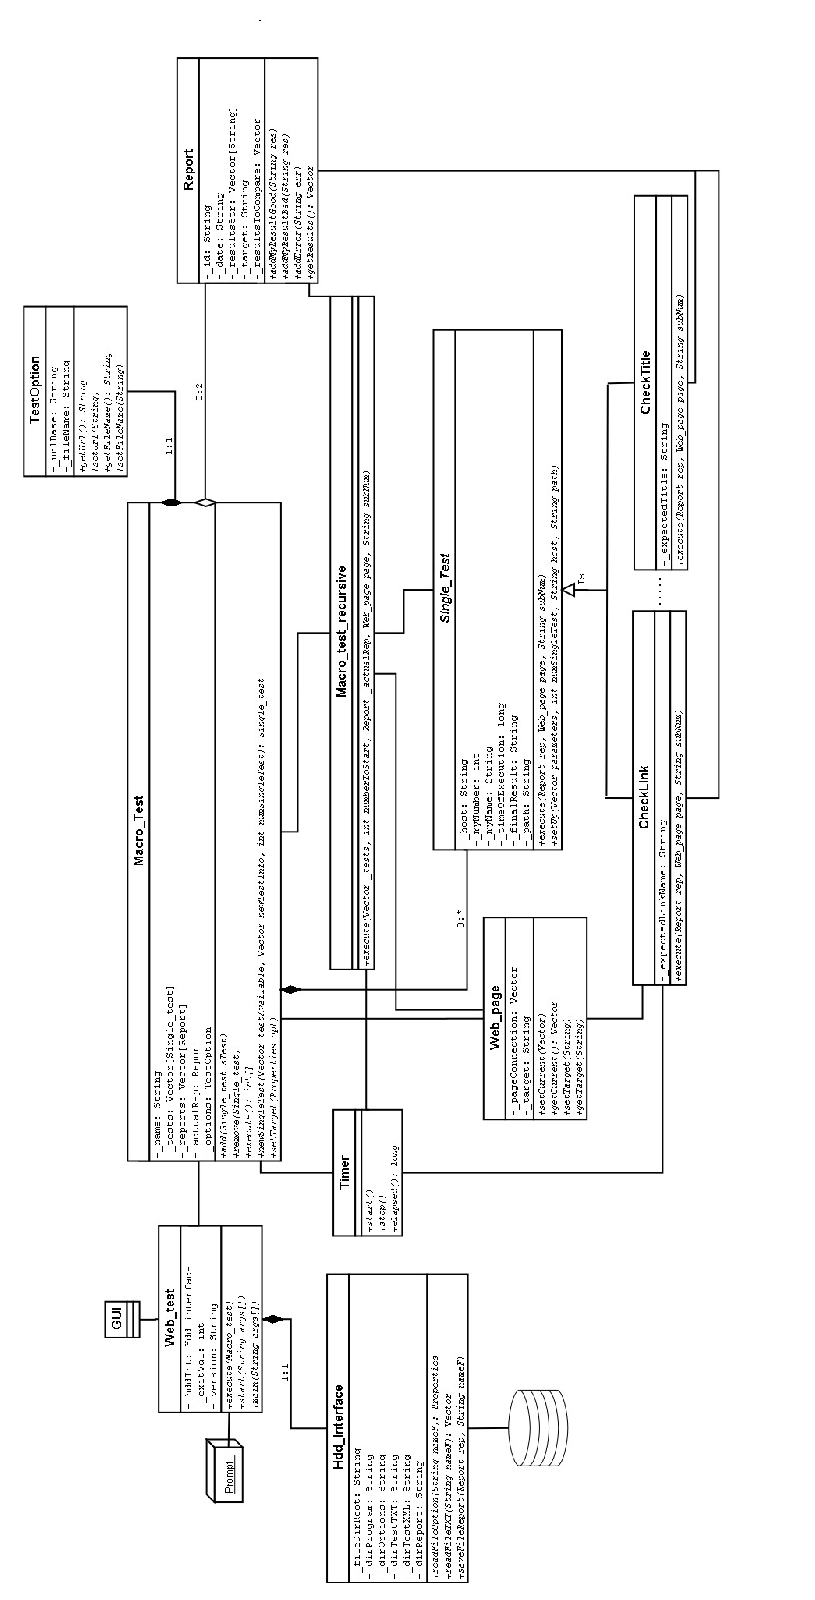
\includegraphics[width=1.0\textwidth , height =	\textheight]{immagini/diagrammaUML.eps}		
	\end{center}
	\caption{Diagramma UML di Bellerofonte}
	\label{fig:diagrammaUML}
\end{figure}

\clearpage

\subsection{Analisi dei metodi pi� significativi}
Entrando un p� pi� nel dettaglio si descrivono ora tre importanti metodi appartenenti alle classi presentate nel paragrafo precedente. 
\begin{itemize}
	\item \emph{Web test.start}: questo � sicuramente il metodo pi� generale. Viene invocato dal main sull'oggetto di classe Web test e coordina tutte le azioni principali svolte durante il test. In input prende il vettore di argomenti passati al programma dalla riga di comando. Se manca un argomento necessario al funzionamento, start lancia una console interattiva che richiede all'utente tutti i parametri necessari oppure fa terminare il programma. In base a questi parametri (nome del file delle opzioni, nome del file test e modalit� di salvataggio del report) start agisce in modi differenti. Provvede anzitutto a richiedere all'Hdd interface il contenuto del file contenente i test singoli attualmente riconosciuti (ovvero le cui classi sono presenti ed istanziabili). Poi crea un oggetto di classe Macro test e gli assegna il nome del file test ricevuto come parametro. Prosegue col richiedere l'elenco delle opzioni all'oggetto Hdd interface, a cui passa il relativo nome di file. Se il file test letto dall'hard disk ha estensione ``.tst'"' significa che � codificato in XML e rappresenta un Macro test precedentemente eseguito e serializzato. Si pu� dunque effettuare una deserializzazione ed un ripristino rapido del suo stato, provvedendo solamente alla sovrascrittura delle opzioni (dato che potrebbero essere cambiate dall'ultima esecuzione). Altrimenti, se il file test ha un'altra estensione (``.txt'"'), start capisce che si tratta di un file di testo che rappresenta un Macro test alla prima esecuzione. Provvede dunque a tradurre l'elenco di direttive ricevute in un oggetto Macro test pronto per essere eseguito: imposta le opzioni, legge i nomi dei test singoli che dovranno comporre il Macro test, li crea e glieli aggiunge. Terminata questa fase preparatoria Macro test viene finalmente eseguito. 
	
Una volta che ogni Single test � terminato (con vario esito) ed ha aggiunto al report il proprio risultato, start cerca nel terzo parametro (opzionale, passatogli dalla riga di comando o dalla console interattiva), le indicazioni su come trattare l'oggetto Macro test ed il relativo report. Prima di terminare start visualizza il conteggio dei test singoli eseguiti, suddividendoli in base all'esito riportato. Bellerofonte si basa poi su questi conteggi per decidere il proprio valore di ritorno al sistema: 0 nel caso in cui ogni Single test sia stato passato, 1 se si � verificato almeno un fallimento e 2 se si � verificato almeno un errore generale;
	
	\item \emph{Macro test.newSingleTest}: questo metodo di Macro test istanzia, a tempo di esecuzione, nuovi oggetti corrispondenti ai test singoli (per esempio CheckTitle), continuando a gestirli tramite la loro classe base: Single test. Viene sfruttato cio� il \emph{polimorfismo},\index{Polimorfismo} una delle caratteristiche principali dei linguaggi orientati agli oggetti. In questo caso ogni test singolo concreto pu� essere istanziato ed utilizzato al posto della classe base astratta Single test, da cui deriva. Nel far ci� i metodi della classe derivata (concreta) si specializzano, sovrascrivendo i metodi della classe base (setUp ed execute principalmente). Macro test, per poter creare test singoli concreti, deve conoscere i nomi delle rispettive classi. Una volta ottenuti i nomi (leggendo da un apposito file di programma), Macro test crea altrettanti oggetti grazie alla \emph{Reflection} di Java. Se per ogni nome di test � stato possibile creare il Single test concreto richiesto, questo � restituito all'ambiente chiamante correttamente inizializzato e pronto per essere eseguito;
	
	\item \emph{Macro test.execute}: l'execute di un Macro test corrisponde all'esecuzione di ogni test singolo presente nel vettore \_tests pi� varie operazioni di coordinamento. Anzitutto viene creato un nuovo Report, che sar� aggiornato in ogni fase dell'elaborazione. In seguito si fa partire il Timer e si cominciano ad eseguire sequenzialmente i test singoli. Ad ogni test singolo viene passato:
	
\begin{itemize}
	\item il riferimento al Report da aggiornare; 
	\item un oggetto Web page al quale riferirsi per i test;
	\item il numero di sequenza del Single test.	
\end{itemize}
Una volta terminata questa fase viene fermato il Timer (rilevando il tempo di esecuzione) e viene ritornato all'ambiente chiamante il numero di test passati, falliti e gli eventuali errori generati.		
\end{itemize}

\subsection{Rassegna dei test base implementati}
Nella versione base di Bellerofonte sono stati realizzati 22 test singoli. Eccoli descritti brevemente (per ulteriori informazioni ci si pu� avvalere del capitolo sei e dei documenti inclusi nel pacchetto orbilio.webTest.bellerofonte):
\begin{enumerate}
	\item \textbf{AddCookie}: con questo test � possibile definire il valore di un cookie da inviare al server per identificare una sessione;
	\item \textbf{CheckButtonValue}: controlla se un form ha un certo pulsante (per esempio ``Submit'"') ed eventualmente lo ``clicca'"';
	\item \textbf{CheckCharacterSet}: controlla il set di caratteri usato in un sito;
	\item \textbf{CheckForm}: controlla se in una pagina � presente un certo form;
	\item \textbf{CheckFormAction}: controlla il valore del parametro ``action'"' di un form;
	\item \textbf{CheckFormContent}: verifica se un form ha un campo con un dato valore;
	\item \textbf{CheckFormField}: verifica la presenza di un campo in un form;
	\item \textbf{CheckFormMethod}: controlla il valore del parametro ``method'"' di un form;
	\item \textbf{CheckImage}: verifica la presenza di un'immagine;
	\item \textbf{CheckLink}: controlla la presenza di un link e la validit� dell'URL associato;
	\item \textbf{CheckMailLinks}: esamina un link ``mailto'"';
	\item \textbf{CheckTable}: verifica la presenza di una data tabella;
	\item \textbf{CheckTableContent}: data una tabella, verifica il contenuto di una sua cella;
	\item \textbf{CheckTextInPage}: data una parola chiave, la ricerca nel testo contenuto in una pagina;
	\item \textbf{CheckTitle}: verifica il titolo della pagina;
	\item \textbf{FollowLinks}: data una stringa od un URL seleziona tutti i link che gli corrispondono e li restituisce a Macro test affinch� li possa seguire;
	\item \textbf{GetFrameContent}: se nella pagina � presente un frame con un dato nome, passa ad esaminarlo;
	\item \textbf{GetHttpHeader}: riporta i contenuti attuali delle intestazioni nei messaggi HTTP;
	\item \textbf{ReachAll}: selezionata una profondit� di visita ed un elenco di pagine da raggiungere, verifica la loro raggiungibilit� effettuando una visita in profondit� del sito. Non segue i link esterni;
	\item \textbf{SetFormContent}: imposta un certo valore in un campo di un form;
	\item \textbf{SubmitForm}: preme il bottone ``Submit'"' di un form e lo invia al server, aggiornando Web page con la risposta ricevuta;
	\item \textbf{UploadFileWithForm}: dato un form in cui � prevista questa funzione, effettua un upload di un file.
\end{enumerate}

%*******************************************************************
\section{Estendere Bellerofonte}
Concepire un software statico, difficilmente estendibile, in un settore tanto mutevole quale � il web testing, � un grave errore di valutazione: troppo arduo pensare di racchiudere in un'unica soluzione ogni possibile test effettuabile, tanto pi� che non si sa cosa dovr� essere testato in futuro. Un software difficilmente estendibile, bench� completo e curato sul momento, rischia di avere vita breve, perch� scarsamente adattabile alle particolari esigenze dei verificatori. Con Bellerofonte non si ha la presunzione di offrire un prodotto ``finito'"', bens� un ``progetto in continua evoluzione'"', capace di integrare con poco sforzo eventuali nuovi test. 

\subsection{Come aggiungere funzionalit� ex-novo}
Aggiungere semplicemente dei test a quelli gi� esistenti, senza portare modifiche strutturali o semantiche alle classi di Bellerofonte, dovrebbe risultare un compito relativamente semplice per degli sviluppatori. Disponendo della directory di lavoro di Bellerofonte (figura \ref{fig:fileProgram}), i passi da eseguire sono standard:
\begin{enumerate}
	\item anzitutto si deve individuare la libreria adatta alla realizzazione del nuovo test: o si sfrutta solo la libreria di default (HTTPUnit) o se ne deve importare (in aggiunta) una nuova. Se la libreria scelta non � compresa da quelle gi� utilizzate in precedenti test allora � necessario:	
\begin{enumerate}
	\item copiare il relativo file jar nella directory /jars;
	\item editare il file manifest.mf in /lib aggiungendo nella riga ``Class-Path'"' la scritta ``../jars/'"' + $<$nome Jar aggiunto$>$	
	\item ricordarsi di aggiungere il nuovo archivio jar nel Path dell'editor usato per scrivere il nuovo test;
\end{enumerate}

\item una volta selezionata una o pi� librerie adatte, aprire il file ``Anonymus.java'"' che si trova in /src e salvare subito con altro nome il nuovo test. Anonymus � semplicemente lo ``scheletro'"' di ogni nuovo test singolo e dovrebbe pertanto rimanere tale;

\item rinominare la nuova classe ed il suo costruttore con il nome del nuovo test. \'E importante che ogni classe test resti estensione di Single test ed implementi l'interfaccia ``Serializable'"';

\item viene adesso la fase pi� complicata. Nella nuova classe test sono individuabili cinque aree personalizzabili. Si deve procedere al loro corretto riempimento evitando di modificare il restante codice, che serve a Bellerofonte per gestire i test singoli a prescindere dalla loro funzione. In un certo senso il programmatore dovr� comportarsi come se stesse sovrascrivendo determinate parti di un'\emph{interfaccia}. Il significato di ogni area � spiegato pi� dettagliatamente nei documenti ``howTo'"' inclusi nella directory /various. Qualora la funzione di un'area non risultasse chiara � consigliabile l'ispezione del listato di qualche altro Single test gi� implementato. \\
Il listato della classe \emph{Anonymus}, cos� come viene trovata dal programmatore nel momento in cui decide di specializzarla in un nuovo test singolo, � presentato di seguito. Le aree sulle quali si dovr� intervenire sono delimitate da apposite stringhe di commento:

\scriptsize
\lstset{language=Java}
\begin{lstlisting}[title={Listato della classe Anonymus.java}, breaklines=true, frame=shadowbox, showspaces=false]

package orbilio.webTest.bellerofonte;

import java.util.Vector;
import java.io.Serializable; 

//////////////// FOLLOWING CAN CHANGE FROM TEST TO TEST 	
import java.net.*;
import java.io.IOException;

// Libraries used
import com.meterware.httpunit.*;
//////////////// END OF COMMON CHANGE AREA 

/**
 * @author Claudio Tortorelli - 2003
 * 
 */
//-----------------------------------------

class Anonymus extends Single_test implements Serializable
{
/**
 * Fields
 */  
 
//////////////// FOLLOWING CAN CHANGE FROM TEST TO TEST 
  private String _expectedInput = "";
//////////////// END OF COMMON CHANGE AREA 	
 	 	
/************************************************
 * Constructor
 */
  public Anonymus()
  {
   super();
  }
/************************************************
 * This setUp method reads an ordered list of 
 * parameters embedded in a Parameters object, some
 * test options and the single test's number. With
 * these informations it intializes its objects.
 *
 * IN: a vector with parameters specified in 
 * macro test file and the number of test. 
 * The vector has at first position the test's
 * name and the other positions hold the actual parameters	
 * OUT: void
 */
  public void setUp(Vector parameters, int numSingleTest) 
  { 			
   _myNumber =  numSingleTest;
   _myName = (String)parameters.elementAt(0); 
   _finalResult = "notCheckedYet";
   _timeOfExecution = "0";
    		
//////////////// FOLLOWING CAN CHANGE FROM TEST TO TEST 	
  //read words from file test txt or xml					
   _expectedInput = (String)parameters.elementAt(1); 
//////////////// END OF COMMON CHANGE AREA 

  }
/************************************************
 * This method implements the particular execution of
 * this single test. It take as parameters the 
 * report and the list of values returned by some
 * eventual previous tests. It returns its values.
 *
 * IN: report for add results, file name target,
 * vector with results of previous test 
 * OUT: vector with the results of this test
 */ 	
  public void execute(Report rep, Web_page page, String subNum) 
  {			
  // strings of header of Single_test	
    String num = _myNumber + subNum;
    String target = page.getTarget();
    String head1 = "TEST: \""+_myName+"\""+" | Url: "+target; 
    rep.addHeader(head1, num);	       
  // start timer
    Timer tim = new Timer();
    tim.start();		    

//////////////// FOLLOWING CAN CHANGE FROM TEST TO TEST 
    rep.addResultExpected("Input: " + _expectedInput);		
//////////////// END OF COMMON CHANGE AREA 

  // get page's state elements, 
  // if 0 then the page was not loaded correctly
    Vector pageData = page.getCurrent();			
    if (pageData.size() != 0)
    {			
    
//////////////// FOLLOWING CAN CHANGE FROM TEST TO TEST 
/* //test passed to Report									
 *  rep.addMyResultGood("The file upload has been setted");  	
 * // don't change: it is used for comparison
 *  _finalResult = "PASSED"; 
 *
 * //test failed to Report									
 *  rep.addMyResultBad("The file upload has been setted"); 
 * // don't change: it is used for comparison
 *  _finalResult = "FAILED"; 
 */			
//////////////// END OF COMMON CHANGE AREA

    }
  // the web page wasn't load correctly
    else
    {			
      rep.addError("Impossible to perform this test");			
      _finalResult = "ERROR";
    }
  // stop timer and set elapsed time		
    tim.stop();		
    long oneSec = 1000;
    _timeOfExecution = tim.elapsed()/oneSec+"."+tim.elapsed();
    rep.addSecOfExecution(_timeOfExecution);
  // add to Report the significative datas 		
    rep.addDataToCompare(_myName, _finalResult, _timeOfExecution);
  // end of execution 
    rep.addSeparation();	
  }		
} // end of class
\end{lstlisting}
\normalsize

\item quando il test realizzato ha complessit� elevata si consiglia di realizzare dei metodi privati interni, da richiamare nelle aree sopra descritte. Come esempio si pu� considerare il metodo \emph{visitDep} del test \emph{ReachAll}. 

Seguendo lo stesso principio, se per realizzare il test si devono implementare svariate classi accessorie, � indicato includerle in un'apposita libreria da inserire assieme agli altri jar nella directory /jars. Anche in questo caso pu� essere preso come esempio ReachAll, per il quale � stata realizzata la libreria claudiosoft.struct.btree;

\item se, al termine dell'attivit� di programmazione, il codice Java del nuovo test compila correttamente, si deve procedere all'aggiunta del file al progetto orbilio.bellerofonte. Una volta effettuato un \emph{rebuild} dell'intero progetto, si deve verificare che l'output della compilazione (ovvero i file ``.class'"' tra cui quello del nuovo test) sia stato correttamente inserito in /orbilio/webTest/bellerofonte. \'E in quella directory che Bellerofonte andr� a cercare la definizione del nuovo test invocabile;

\item si procede poi ad editare il file ``TestList.txt'"' contenuto in /webtestfiles/program. Esso contiene un elenco dei nomi di tutti i Single test per i quali esiste una definizione. Per aggiornarlo basta aggiungere in fondo alla lista dei test attualmente riconosciuti, il nome del nuovo test creato. \'E importante che sia rispettata l'esatta sequenza di maiuscole e minuscole;

\item editare anche il file ``TestSynopsis.txt'"' in /webTestFiles/program (e il suo omologo ``.doc'"' in /various) aggiungendo l'esatta segnatura ed una sintetica descrizione del nuovo test. Ci� non � strettamente necessario al funzionamento del software, ma � richiesto per lasciare una minima documentazione sui nuovi test introdotti.

\item eseguire infine lo script batch ``makeJar.bat'"' in /bin, il quale provvede automaticamente ad:
\begin{itemize}
	\item aggiornare il file ``Bellerofonte.jar'"' in /lib aggiungendo il nuovo file ``.class'"';
	\item aggiungere alla variabile di sistema Classpath il nome di eventuali nuovi archivi jar inseriti in /jars.
\end{itemize}
\end{enumerate}

\subsection{Possibili sviluppi futuri}
Attualmente Bellerofonte non dispone di un'adeguata interfaccia grafica (Pegaso) che dovrebbe supportare l'utente durante tutta le fasi di preparazione ed esecuzione del test descritte nel prossimo capitolo. 

Un'altra mancanza che si potrebbe pensare di colmare � l'impossibilit� di effettuare test di performance e stress. Essendo per� Bellerofonte richiamabile dalla riga di comando, � piuttosto semplice creare uno script esterno che includa una sua esecuzione separata in $n$ \emph{thread} diversi. D'altro canto, Bellerofonte � stato progettato principalmente in funzione di Orbilio, applicazione che attualmente non ha bisogno di simili test. 

Altri aspetti che meriterebbero maggiore attenzione in versioni future di Bellerofonte potrebbero essere:
\begin{itemize}
	\item ottimizzazione del disegno e del codice;
	\item migliore gestione dei report;
	\item migliore gestione del timer;
	\item utilizzo pi� raffinato dell'XML nella definizione dei Macro test;
	\item inserimento di test pi� sicuri nell'analisi degli script;
	\item considerare specifici test di usabilit�, quali quelli che verificano l'accessibilit� per utenti disabili.
\end{itemize}

%----------------------------------------------------------------
\chapter{Manuale d'uso}

In questo capitolo verranno illustrate le procedure di utilizzo di Bellerofonte. Prima per� � bene chiarire quali sono e come sono strutturati i file e le directory usate dal programma. 

\section{File di programma}
Bellerofonte presume di lavorare sempre all'interno di un sistema predefinito di file e directory rappresentato in figura \ref{fig:fileProgram}.

\begin{figure}[bp]
	\begin{center}
		\includegraphics[width=.7\textwidth, height = 	0.7\textheight]{immagini/fileProgram.eps}		
	\end{center}		
	\caption{Directory di lavoro di Bellerofonte}	
	\label{fig:fileProgram}
\end{figure}

Il programma fa sempre riferimento alla directory webTestFile come propria \emph{root}, la quale a sua volta ha cinque sottodirectory: 
\begin{itemize}
	\item \emph{options}: contiene i file che specificano le impostazioni per l'esecuzione dei file test;
	\item \emph{program}: vi sono i file necessari al programma (e agli utenti) per riconoscere i test singoli attualmente disponibili;
	\item \emph{reports}: qui sono salvati i report in formato testo;
	\item \emph{testTXT}: in questa cartella ci sono i file test in formato testo. Ognuno di essi rappresenta un Macro test da assemblare sulla base delle direttive lette da file. Il verificatore, nel preparare un nuovo test, si concentrer� prevalentemente su questi file. 
	\item \emph{testXML}: gli oggetti Macro\_test serializzati, insieme ai propri report, vengono salvati in questa directory in formato XML. L'estensione dei file XML � ``.tst'"' ed il verificatore pu� leggerli ed eventualmente editarli con qualunque editor di testo o browser. La differenza tra i file test ``.txt'"' e quelli ``.tst'"' verr� illustrata tra breve.
\end{itemize}

Oltre alla directory webTestFile, all'interno del pacchetto ci sono altre directory di cui Bellerofonte non ha stretto bisogno ma che lo rendono pi� usabile:
\begin{itemize}
	\item \textbf{bin}: contiene degli script batch che ne agevolano l'uso e il mantenimento. 	
\begin{enumerate}
	\item ``belJAR.bat'"', quando viene avviato, va ad eseguire l'archivio jar contenente Bellerofonte. Questo script pu� essere invocato sia da ambiente DOS/Windows che da Unix (cambiandone i permessi di esecuzione), passandogli o meno i parametri che richiede Bellerofonte. Provvede infatti lo stesso Bellerofonte ad avviare un processo interattivo che interroga l'utente sugli input mancanti. Per questa particolarit�, belJar � adatto ad essere richiamato anche da un ambiente a finestre, semplicemente cliccandoci sopra;
	\item ``makeJar.bat'"' ha una funzione accessoria, utile agli sviluppatori di nuovi test singoli: esso aggiorna automaticamente l'archivio eseguibile ``bellerofonte.jar'"' con tutte le nuove definizioni ``.class'"' trovate. Per far questo va a leggere il file ``manifest.mf'"', dove tra l'altro viene impostata la variabile di ambiente ``Classpath'"' affinch� Bellerofonte sappia dove trovare le varie librerie jar usate dai test singoli.
\end{enumerate}

	\item \textbf{jars}: questa directory contiene gli archivi jar compressi con i pacchetti utilizzati nei Single test o da Bellerofonte;
	
	\item \textbf{lib}: dentro lib si trova il jar eseguibile ``bellerofonte.jar'"' ed il relativo file ``manifest.mf'"';
	
	\item \textbf{orbilio$\backslash$webTest$\backslash$bellerofonte}: qui viene aggiornato l'output della compilazione dei file sorgenti. Vi sono i file ``.class'"' delle classi di programma e dei vari test singoli. Bellerofonte controlla in questa directory la presenza delle definizioni dei test singoli prima di istanziarne gli oggetti;
	
	\item \textbf{src}: in src stanno i file ``.java'"' ovvero i sorgenti di Bellerofonte e dei Single test;
	
	\item \textbf{various}: in various sono stati inseriti i file di documentazione insieme ad immagini significative (come quelle che appaiono in questa tesi). In particolare sono presenti (in vari formati) documenti per l'utilizzo e l'estensione di Bellerofonte e le sue API in formato HTML.
\end{itemize}

\section{Eseguire Bellerofonte}
Illustrato l'ambiente nel quale ci si dovr� muovere, si pu� procedere col descrivere come eseguire Bellerofonte, soffermandosi su come accedere alle sue funzionalit� e senza entrare nuovamente nei dettagli della loro implementazione. 
Bellerofonte ha bisogno di alcuni parametri in input per essere eseguito:
\begin{itemize}
	\item il nome di un file opzioni;
	\item il nome di un file test;
	\item una parola chiave che lo istruisca su come trattare il report ed il Macro test eseguito. 
\end{itemize}
Come gi� si � detto nel capitolo precedente, i primi due valori sono necessari mentre il terzo � opzionale. Spostandosi nella cartella bin, la sintassi di esecuzione dalla riga di comando � la seguente:

\footnotesize
\begin{verbatim}
belJar <OPZIONI.txt> [<TEST.txt>|<TEST.tst>]
(saveToMacroTest|compareToOld|compareToOldAndSave|<REPORT.txt>|<NULL>)
\end{verbatim}
\normalsize
oppure semplicemente
\footnotesize
\begin{verbatim}
belJar 
\end{verbatim}
\normalsize
In ogni caso � necessario preparare i file di cui il software fa richiesta prima dell'esecuzione. Bellerofonte li andr� a ricercare solo ed esclusivamente nelle directory predefinite. 

\subsection{Preparare il file opzioni}
Il primo parametro obbligatorio da preparare � il file di opzioni. Questi file possono essere editati dall'utente nella directory webTestFiles$\backslash$options con un qualsiasi editor di testo. La forma che deve avere un file opzioni � quella tipica dei \emph{file Properties} di Java, in cui si ha una serie di coppie \emph{chiave $=$ valore}. Le scelte selezionabili in ognuno di questi file sono numerose e suddivise in tre categorie:
\begin{itemize}
	\item Target options: descrivono il \emph{target} del test, ovvero l'indirizzo dal quale il test dovr� partire;
	\item Client options: definiscono l'identit� e le funzionalit� generali del client, nella fattispecie Bellerofonte stesso;
	\item HTTPUnit options: sono pi� strettamente legate alle modalit� di rappresentazione degli oggetti web incontrati da parte di HTTPUnit.
\end{itemize}
La maggioranza delle scelte non ha bisogno di modifiche da parte del verificatore (se non per particolari tipi di test), ma � ovviamente obbligatorio inserire almeno un target raggiungibile.
Un esempio di file opzioni ``pulito'"' (cio� non relativo a nessun sito testato) � ``options.txt'"', che si consiglia di utilizzare come modello (salvandolo quindi con un nuovo nome).
Si � scelto di imporre la definizione separata dei file opzioni rispetto ai Macro test in quanto si suppone che il verificatore, oltre a crearsi una propria libreria di file test, realizzi anche un certo numero di opzioni relative ai siti da verificare. Ognuno di questi file sar� poi indipendente e combinabile liberamente con i file test.

Dato che l'attuale versione di HTTPUnit ha mostrato problemi ad interpretare alcuni linguaggi di scripting, una soluzione � quella di disabilitare, quando necessario, il parsing di tali linguaggi. Per ulteriori informazioni e aggiornamenti su questa lacuna di HTTPUnit si rimanda al suo sito web.

\subsection{Preparare il file test}
La fase successiva � quella di definizione del Macro test in un file test. I file test possono avere due forme e due ruoli diversi:
\begin{itemize}
	\item Nel primo caso si suppone che il verificatore debba comporre un nuovo Macro test. Un nuovo Macro test viene descritto a partire da un file di testo in cui si elencano ordinatamente i nomi ed i parametri di ogni test singolo, separati dal carattere `$\mid$'.
La sintassi di ogni riga di un file test � quindi 

\footnotesize
\begin{verbatim}
<NOME SINGLE TEST>|*(PARAMETRO N-ESIMO|)
\end{verbatim}
\normalsize
L'elenco dei test singoli con la loro sintassi e la semantica dei parametri � inserito nei file ``TestSynopsis.txt'"' e ``TestSynopsis.doc'"' (presente anche in formato pdf). Il verificatore pu� trovare degli esempi e prenderli come punto di partenza per i propri test in webTestFiles$\backslash$testTXT. 

La definizione di un Macro test tramite file di testo implica la creazione di un nuovo oggetto Macro\_test all'interno di Bellerofonte. Questa osservazione � importante quando si devono gestire i salvataggi: se partendo da un file di testo era gi� stato salvato un oggetto Macro\_test in precedenza e questo conteneva dei report relativi a passate esecuzioni, l'aver forzato Bellerofonte a ricostruire un nuovo (ma omonimo) Macro\_test provoca una sovrascrittura, con conseguente perdita dei report gi� salvati. 

Nell'editare un file di test ci si deve ricordare che quel che si scrive � \emph{case sensitive}, ovvero Bellerofonte � sensibile alla differenza tra maiuscole e minuscole. Riguardo ai parametri che seguono il nome c'� da dire che essi vengono di solito trattati tutti come stringhe e solo i Single test che ne fanno un uso particolare li convertono, dove serve, in valori numerici. I parametri, essendo delle stringhe, comprendono ogni carattere tra due delimitatori $\mid$ (spazi inclusi). Bisogna inoltre stare attenti a non lasciare righe vuote nel file test, che Bellerofonte potrebbe tradurre in modo imprevedibile. Un file test vuoto invece corrisponde ad un Macro test nullo. 

Un file test ha pressappoco la funzione del test script, ovvero ordina e definisce i passi di un test riferito ad una singola caratteristica del sito. Tutti i test singoli che sono inseriti in un file test dovrebbero quindi concorrere alla verifica di un unico aspetto. Per questo se un test singolo effettua una modifica sull'oggetto che testa, influisce sulle esecuzioni dei test seguenti. 

Un semplice esempio di file test in formato testo � il seguente:
\footnotesize
\begin{verbatim}
FollowLinks|string|Home|
CheckTitle|My HomePage|
\end{verbatim}
\normalsize

	\item L'alternativa, citata in precedenza, alla definizione di un Macro test con un file di testo � quella di riutilizzare un oggetto XML serializzato, contenente un Macro\_test gi� definito. In pratica la serializzazione comprende il salvataggio dello stato dell'oggetto Macro\_test al termine della sua esecuzione: si memorizza il vettore dei Single test gi� costruito, il report attuale e le opzioni inizializzate (bench� queste saranno comunque rilette e sovrascritte in successive esecuzioni). Un Macro test serializzato costituisce quindi un oggetto pronto per essere rieseguito, con in pi� la capacit� di memorizzare e comparare i risultati delle sue esecuzioni. Altri due vantaggi dell'utilizzo di un file ``.tst'"', sono la maggior rapidit� di esecuzione e la possibilit� di visualizzare e modificare oggetti serializzati, perch� codificati nell'ormai universale XML.
Si deve per� ricordare che un verificatore non pu� direttamente definire un oggetto di questo tipo. Esso deve necessariamente passare attraverso un Macro test su file di testo, il quale potr� essere serializzato in seguito alla sua prima esecuzione. Esempi di file ``.tst'"' si trovano nella cartella webTestFiles$\backslash$testXML.

\end{itemize}
  
\subsection{Gestire i risultati}
Il terzo aspetto, opzionale ma propedeutico all'esecuzione di un Macro test, � quello che riguarda la gestione dei risultati, ovvero del report e dell'oggetto Macro\_test. A seconda di quale parola chiave compaia come terzo parametro, Bellerofonte agisce di conseguenza:
\begin{itemize}
	\item nel caso in cui nessuna stringa segua i nomi dei file opzioni e test, il programma semplicemente termina subito dopo aver eseguito il Macro test specificato (restituendo cio� solamente i risultati a video);
	\item quando compare qualsiasi stringa diversa dalle parole chiave riconosciute, il software la interpreta come nome di un file di testo. Tale file sar� usato per salvare il contenuto del report attuale nell'apposita directory webTestFile$\backslash$reports;
	\item inserendo la parola chiave \emph{``saveToMacroTest'"'} Bellerofonte serializzer� il Macro\_test ed il report attuali in un file XML con estensione ``.tst'"' nella directory webTestFiles$\backslash$testXML. ``saveToMacroTest'"' pu� produrre effetti molto differenti: 
\begin{enumerate}
	\item se il Macro test viene letto da un file di testo e gi� esisteva un oggetto serializzato, questo viene sovrascritto (con conseguente cancellazione dei report contenuti);
	\item altrimenti se viene letto da un file ``.tst'"', ``saveToMacroTest'"' provoca un salvataggio del report attuale nello stesso file XML. Un oggetto ``.tst'"' pu� contenere al massimo gli ultimi due report realizzati. Il salvataggio di un terzo report coincide con la cancellazione di quello pi� vecchio;
\end{enumerate}
	 
	\item la parola chiave \emph{``compareToOld'"'} non implica il salvataggio del report attuale ma il confronto a video con i report precedenti. Questo parametro viene preso in considerazione da Bellerofonte solo se associato ad un Macro test gi� eseguito (quindi contenuto in un file ``.tst'"'). Attualmente non � previsto il salvataggio su file delle schermate di comparazione;
	\item infine \emph{``compareToOldAndSave'"'}  provoca l'ovvia somma degli effetti delle due parole chiave precedenti. Si provvede a salvare il nuovo report sull'oggetto XML serializzato ed al tempo stesso si restituisce a video la sua comparazione con i due ultimi report salvati. Anche questa variante presuppone la lettura del Macro test da un file ``.tst'"'.
\end{itemize}
In ogni caso il programma accetta i parametri solo nell'ordine stabilito e le parole chiave illustrate in questa sezione si escludono a vicenda.

\subsection{La console interattiva}
La console interattiva consente al verificatore di avere sotto controllo tutti i file (opzioni, ``.txt'"' e ``.tst'"') fino a quel momento creati. Infatti Bellerofonte, nel richiedere i parametri di input, presenta a video un elenco degli oggetti contenuti nelle directory delle opzioni e dei test, cos� che l'utente possa selezionarli semplicemente digitandone il numero progressivo. Qualora questo numero non fosse inserito oppure non corrispondesse a nessun file, il programma terminerebbe chiudendo la console e senza eseguire alcun test. 

Il verificatore pu� rispondere alle richieste della console anche digitando per intero (cio� compresa l'estensione) il nome dei file. Invece, nella terza domanda relativa alle parole chiave, la stringa introdotta come nome di file report viene automaticamente completata con l'estensione ``.txt'"' quando questa sia stata omessa.

Se per mancanza degli input dalla riga di comando Bellerofonte � costretto ad avviare la console interattiva, la terminazione del programma dovr� essere preceduta dalla pressione del tasto ``Invio'"'.

\subsection{Esempi pratici}
Per concludere questo capitolo sull'uso pratico di Bellerofonte, si riportano alcuni esempi:
\begin{enumerate}
	\item \textbf{Verifica di un sito con parametri dalla riga di comando}:
\begin{verbatim}
 beljar orbilioLocal.txt testprova3.txt 
\end{verbatim}
\normalsize
\textbf{Output}:
\scriptsize
	\begin{lstlisting}	
C:\claudiosoft.bellerofonte\bin>echo off 

Bellerofonte: ver. 1.0 --- 2-ago-2003 11.41.12
 
-----------------------------------------------------
REPORT OF TEST: testprova3.txt - 2-ago-2003 11.41.12
-----------------------------------------------------
 
1.0] TEST: "SetFormContent" | Url: http://127.0.0.1/index.php
   Result expected: "Form: 0"
   Result expected: "Field: uname"
   Result expected: "Value to set: u1"
   + TEST PASSED: The field has been setted at the expected value
 
   # Seconds elapsed to accomplish the test: 0.10
 
/\/\/\/\/\/\/\/\/\/\/\/\/\/\/\/\/\/\/\/\/\/\/\/\/\/\
 
2.0] TEST: "SetFormContent" | Url: http://127.0.0.1/index.php
   Result expected: "Form: 0"
   Result expected: "Field: pass"
   Result expected: "Value to set: u1"
   + TEST PASSED: The field has been setted at the expected value
 
   # Seconds elapsed to accomplish the test: 0.0
 
/\/\/\/\/\/\/\/\/\/\/\/\/\/\/\/\/\/\/\/\/\/\/\/\/\/\
 
3.0] TEST: "SubmitForm" | Url: http://127.0.0.1/index.php
   Result expected: "Form: 0"
   Result expected: "Button: "
   + TEST PASSED: Button found and form submitted
 
   # Seconds elapsed to accomplish the test: 0.551
 
/\/\/\/\/\/\/\/\/\/\/\/\/\/\/\/\/\/\/\/\/\/\/\/\/\/\
 
Total seconds of execution: 0.561


Result of tests in testprova3.txt:
  * 3 tests PASSED;
  * 0 tests FAILED;
  * 0 GENERAL ERRORS;
\end{lstlisting}
\normalsize	
	
	\item \textbf{Verifica di un sito con uso di console interattiva}:
\begin{verbatim}
beljar 
\end{verbatim}
\textbf{Output}:
\scriptsize
\begin{lstlisting}	
C:\claudiosoft.bellerofonte\bin>echo off 
 
Bellerofonte: ver. 1.0 --- 2-ago-2003 11.53.54
  
* Write the name of options file that will be used from list below:
 
0- options.txt
1- orbilioLocal.txt
2- orbilioThen.txt
3- otherLocal.txt
4- otherWWW.txt
 
* Write the name of test file that will be used from list below:
 
0- nullTest.txt
1- testButtonValue.txt
2- testFormField.txt
3- testImage.txt
4- testLink.txt
5- testProva.txt
6- testProva2.txt
7- testProva3.txt
8- testSubmit.txt
9- testTitle.txt
10- videoCall.txt
11- testLink.tst
 
* How must the report be treated ?
[1] "saveToMacroTest"
[2] "compareToOld"
[3] "compareToOldAndSave"
- nameReportInTXT
- null
  
  
  
-----------------------------------------------------
REPORT OF TEST: testFormField.txt - 2-ago-2003 11.54.03
-----------------------------------------------------
 
1.0] TEST: "CheckFormField" | Url: http://127.0.0.1/index.php
   Result expected: "Form: 0"
   Result expected: "Field: uname"
   + TEST PASSED: The form has the field expected
 
   # Seconds elapsed to accomplish the test: 0.10
 
/\/\/\/\/\/\/\/\/\/\/\/\/\/\/\/\/\/\/\/\/\/\/\/\/\/\
 
Total seconds of execution: 0.10 
 
Result of tests in testFormField.txt:
  * 1 tests PASSED;
  * 0 tests FAILED;
  * 0 GENERAL ERRORS;
 
(press Enter) --- 2-ago-2003 11.54.06
\end{lstlisting}
\normalsize
	
	\item \textbf{Comparazione tra due report di un Macro test gi� serializzato in precedenza}:
\begin{verbatim}
beljar orbiliolocal.txt testFormField.tst compareToOld
\end{verbatim}	

\textbf{Output}:
\scriptsize
\begin{lstlisting}		
C:\claudiosoft.bellerofonte\bin>echo off 

Bellerofonte: ver. 1.0 --- 2-ago-2003 14.14.04
 
-----------------------------------------------------
REPORT OF TEST: testFormField.txt - 2-ago-2003 14.14.06
-----------------------------------------------------
 
1.0] TEST: "CheckFormField" | Url: http://127.0.0.1/index.php
   Result expected: "Form: 0"
   Result expected: "Field: uname"
   + TEST PASSED: The form has the field expected 
   
 # Seconds elapsed to accomplish the test: 0.0
 
/\/\/\/\/\/\/\/\/\/\/\/\/\/\/\/\/\/\/\/\/\/\/\/\/\/\
 
Total seconds of execution: 0.10

COMPARISON BETWEEN LAST TESTS (Actual Test , Old Test , Very Old Test)
---------------------------------------------------------------------
CheckFormField , CheckFormField
- - - - - - - - - - - - - - - - - - - - - - - - - - 
PASSED , PASSED
- - - - - - - - - - - - - - - - - - - - - - - - - - 
0.20 , 0.10
----------------------------------------------------

Result of tests in testFormField.txt:
  * 1 tests PASSED;
  * 0 tests FAILED;
  * 0 GENERAL ERRORS;
\end{lstlisting}
\normalsize
	\item \textbf{Applicazione di Bellerofonte in vari test consecutivi, a formare una test suite}:
\begin{verbatim}
beljar orbiliolocal.txt testprova2.txt saveToMacroTest | 
beljar orbiliolocal.txt testprova3.txt rep2.txt
\end{verbatim}
In questo caso il risultato � la visualizzazione a schermo dell'ultimo report compilato (``rep2.txt'"'), il suo salvataggio come file di testo nella cartella webTestFiles$\backslash$reports e la serializzazione del file di test ``testprova2.txt'"' nella directory webTestFiles$\backslash$testXML;	
\end{enumerate}




%################################################################
\part{La piattaforma Orbilio: sviluppo e testing}
%################################################################
\chapter{Breve descrizione di Orbilio}
In questo capitolo verr� descritta sommariamente l'applicazione web per la quale Bellerofonte � stato ideato e realizzato: Orbilio. 

Orbilio nasce e si sviluppa all'interno del Dipartimento di Sistemi ed Informatica dell'Universit� di Firenze ed � attualmente seguito da un apposito gruppo di lavoro formato da professori e studenti. 

Esso si propone come strumento di supporto alla didattica e, andando oltre, come piattaforma di \emph{e-learning}, in grado di offrire funzionalit� per l'interazione in tempo reale. Prima di Orbilio, il sito web del Dipartimento (all'URL \textbf{if.dsi.unifi.it}) gi� gestiva una serie di servizi tesi a raccogliere informazioni utili per i professori e fornire un riferimento ai vari corsi per gli studenti. C'era per� l'esigenza di uniformare questi servizi in una piattaforma definitiva, che offrisse, per ogni corso universitario, una comune veste grafica ed un'omogenea implementazione funzionale. 

Dopo aver ispezionato varie alternative presenti attualmente nel ramo del supporto alla didattica, � stata scelta come piattaforma di partenza \emph{Claroline}\index{Claroline}, un'applicazione realizzata all'Universit� Cattolica di Lovanio, in Belgio.
Claroline presenta alcune evidenti qualit�:
\begin{enumerate}
	\item � un progetto con licenza Open Source, ovvero permette la modifica e la successiva redistribuzione dei file sorgenti;
	\item � un software sviluppato sulla base di tre tecnologie molto diffuse e conosciute: il linguaggio PHP, il server Apache ed una base di dati MySQL;
	\item presenta gi� tutta una serie di servizi di base disponibili ai professori ed agli studenti: una \emph{home page} separata e personalizzabile per ogni corso, la gestione di gruppi di lavoro, forum e cos� via.
\end{enumerate}
Dopo un certo periodo di prova sul sito del Dipartimento sono per� emersi anche i limiti e le lacune di questo software:
\begin{itemize}
	\item bench� supporti molte lingue diverse nell'interfaccia, la gestione delle traduzioni non � risultata abbastanza precisa;
	\item il codice sorgente appare caotico e dunque difficile da modificare. Allo sviluppo di Claroline devono aver preso parte, in momenti differenti, persone di varia lingua. Il risultato � una certa ambiguit� nelle definizioni, dovuta prevalentemente alle discrepanze linguistiche e stilistiche in commenti, nomi di variabile, campi del database ed altro ancora;
	\item le modalit� di gestione del database subiscono frequenti modifiche. Ci� si ripercuote direttamente sulla complessit� degli aggiornamenti da una versione all'altra;
	\item gli aspetti amministrativi della piattaforma nel suo complesso non sono sufficientemente flessibili e semplici. Non dispongono inoltre di nessun meccanismo in grado di evitare involontari interventi manuali dannosi.
\end{itemize}
Sulla base di queste constatazioni � stato deciso dal gruppo di lavoro sopra menzionato di effettuare un \emph{fork} dalla piattaforma Claroline ad una nuova piattaforma: Orbilio. Le modifiche da apportare erano in effetti troppe per essere gestite sempre all'interno del progetto Claroline. Inoltre, alla base di Orbilio, sta la volont� di offrire una vera piattaforma di e-learning, cosa che Claroline non mirava ad essere.

Cos� in Orbilio sono stati migliorati o aggiunti i seguenti aspetti:
\begin{itemize}
	\item eliminazione di alcuni file non pi� utilizzati in Claroline, ma comunque compresi nel pacchetto. Il risultato � una maggiore snellezza del progetto;
	\item introduzione di nuove componenti. L'innovazione pi� importante, primo passo verso la realizzazione di una piattaforma di e-learning, � stata l'aggiunta della funzionalit� di \emph{video-ricevimento}, in grado di fornire un contatto diretto tra professore e studenti tramite \emph{web-cam};
	\item integrata una nuova \emph{procedura di autenticazione}\cite{3.5}, capace di rendere effettiva la corrispondenza tra i reali studenti del corso di laurea e gli studenti registrati ad Orbilio nonch� di semplificare le operazioni di gestione;
	\item migliorato l'\emph{aspetto amministrativo}, con aggiunta di nuove schermate di configurazione guidata e gestione assistita del database.		
\end{itemize}
Orbilio punta inoltre ad essere maggiormente usabile ed installabile anche da utenti con scarse conoscenze informatiche. Questo per favorire la sua diffusione anche al di fuori del Dipartimento. Orbilio rimane comunque un progetto Open Source. Per informazioni pi� approfondite sulle piattaforme di e-learning in generale e su Orbilio in particolare si vedano i documenti \cite{3.3} e \cite{3.4} citati in bibliografia. 

%----------------------------------------------------------------
\chapter{Testing di Orbilio con Bellerofonte}
Parallelo al progetto Orbilio descritto nel capitolo precedente, si � sviluppato Bellerofonte. Essendo Orbilio nato da oggettive necessit� di modificare aspetti lacunosi della piattaforma Claroline, si � resa subito palese l'esigenza di garantire uno standard di qualit� minimo nelle modifiche introdotte. Non si voleva infatti ripetere l'errore fatto in Claroline, dove numerose aggiunte di funzionalit� incoerenti tra loro hanno portato ad una confusione diffusa a tutti i livelli ed a un'usabilit� ridotta. 

Bellerofonte � quindi rivolto specialmente ai futuri sviluppatori di Orbilio, i quali, ampliando le funzionalit� della piattaforma con nuovi servizi, saranno chiamati a garantirne la correttezza tramite appositi test. 

\spazioVer
In questa prima versione di Bellerofonte � stata presentata una serie di test singoli i quali, una volta combinati tra loro, possono fornire un'adeguata gamma di test funzionali, regressivi, di caricamento e di interfaccia. Le modalit� con cui realizzare tali test sono quelle illustrate nel capitolo 6. 

Sempre nell'ambito di questa tesi � stato realizzato un semplice test che verifica la raggiungibilit� di un certo numero di file di Orbilio, una volta terminata la procedura di installazione. Questo test, basato sul test singolo ``ReachAll'"', pu� dunque considerarsi un primo esempio di Installation test. 

\section{Un semplice esempio di Installation test}
Orbilio punta ad essere una piattaforma \emph{user-friendly} non solo dal lato dell'utente, ma anche da quello dell'amministratore. \'E una qualit� fondamentale di quei software che ambiscono ad uscire dall'ambiente in cui sono stati creati per essere installati ed usati anche da persone non addette. Per questo motivo, tra i vari test che potevano essere realizzati, se ne � privilegiato uno post-installazione, che consentisse ad un amministratore di controllare automaticamente lo stato della piattaforma appena installata (senza per� includere obbligatoriamente questa verifica in Orbilio). Al tempo stesso si � voluta mostrare la versatilit� di Bellerofonte e la sua capacit� di integrarsi con interfacce grafiche esterne. Il risultato ottenuto conferma queste propriet�, ma, come lo stesso Bellerofonte, non punta ad essere definitivo e rimane suscettibile alle future modifiche di Orbilio. 

In questo paragrafo non si scender� in nessun dettaglio tecnico circa la realizzazione dell'interfaccia grafica che coordina la raccolta dei dati e l'esecuzione del test. Ci� perch� questa particolare implementazione non � rilevante per il web testing e non � neppure vincolante ai fini di future interfacce grafiche di Bellerofonte (la gi� citata Pegaso). La scelta, in questo caso, � caduta su \emph{Swing} di Java per vari motivi:
\begin{itemize}
	\item si integra perfettamente con Bellerofonte sotto molti aspetti: quello tecnico e quello della portabilit� in primo luogo;
	\item c'� un'ampia gamma di componenti e di strumenti per il disegno di interfacce gi� pronti;
	\item consente di creare un'interfaccia \emph{stand-alone}, che cio� ha bisogno solo della Java Virtual Machine per funzionare. 
\end{itemize}
I requisiti quindi coincidono con quelli di Bellerofonte.

L'interfaccia realizzata per l'installation test, che si presenta una volta lanciato il file batch ``TestGUI.bat'"', � mostrata in figura \ref{fig:GUI}

\begin{figure}[bp]
	\begin{center}
		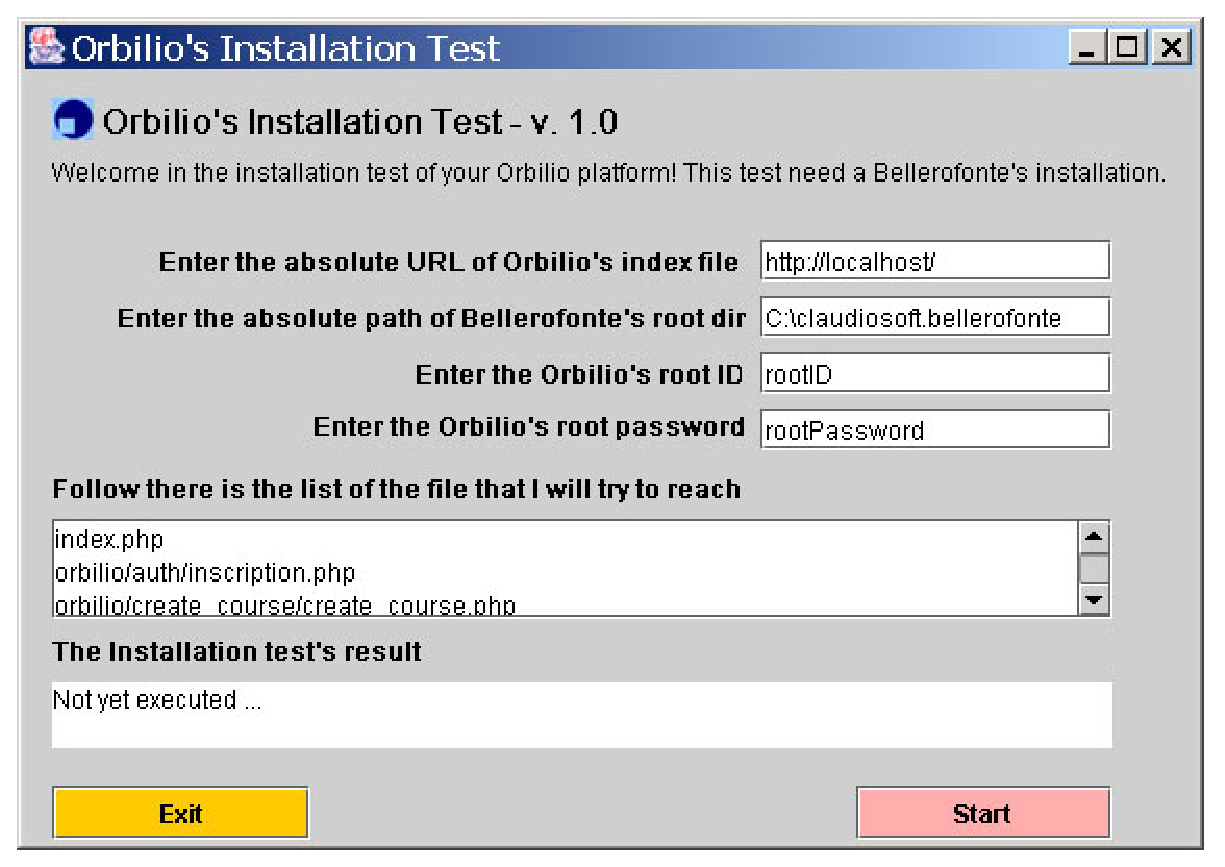
\includegraphics[width=1.0\textwidth, height = 9.5cm]{immagini/GUI.eps}		
	\end{center}			
	\caption{Interfaccia dell'Installation test}	
	\label{fig:GUI}
\end{figure}

L'installation test presume, ovviamente, la disponibilit� di Bellerofonte e di Orbilio. \'E dunque mostrato a chi esegue il test un form nel quale dovranno essere inseriti i seguenti dati:
\begin{enumerate}
	\item l'URL di Orbilio, ovvero della directory dove � collocato il suo ``index.php'"';
	\item il path assoluto della root di Bellerofonte, cio� il percorso nel file system che porta alla directory ``claudiosoft.bellerofonte'"';
	\item l'identificatore di login e la password per accedere ad Orbilio come amministratore.
\end{enumerate}
Al di sotto dei campi citati c'� un'area di testo con i file standard di Orbilio (versione 1.0) che Bellerofonte tenter� di raggiungere nel suo test. A questo elenco di file l'amministratore (o pi� facilmente lo sviluppatore) di Orbilio pu� aggiungerne altri. Se si volesse rendere permanente questa selezione si dovrebbe invece intervenire sul file di testo ``listFile.txt'"' contenuto nella directory ``files'"' della directory ``claudiosoft.testGUI'"'.

L'interfaccia raccoglie tutti i dati (effettuando anche delle verifiche sulla loro correttezza) e, dopo la pressione del bottone ``Start'"', li rielabora: crea il file di opzioni, i file (usati nei test ``ReachAll'"') contenenti gli URL delle pagine da raggiungere ed il file  con l'elenco dei test singoli (in formato testo).

Tutti i file creati, a parte il report, sono temporanei e vengono cancellati all'uscita dal test.

Al termine della fase preparatoria, se non sono state incontrate difficolt�, viene lanciata l'esecuzione di Bellerofonte in un processo separato. L'output di esecuzione scorrer� nella shell mentre il report verr� visualizzato in una finestra \emph{pop-up} aperta appositamente. In base al valore di uscita del sottoprocesso l'interfaccia si aggiorner� di conseguenza, confermando o smentendo al verificatore il buon funzionamento di Orbilio. 

Il test assemblato dell'interfaccia non fornisce in realt� una prova ``forte'"' della corretta installazione di Orbilio: esso � costituito da due esecuzioni separate del test singolo ``ReachAll'"'; la prima � volta a verificare le pagine di base mentre la seconda viene lanciata all'interno dell'area di amministrazione (per questo servono identificatore e password di amministratore). Dato che il test non interessa le funzionalit� ma solo la raggiungibilit� delle pagine elencate, ci si deve accontentare di dedurre che ogni link � funzionante e dunque presumibilmente il web server e il database sono ben configurati. Del resto si pu� ipotizzare che la verifica delle singole componenti sia stata gi� fatta dagli sviluppatori con appositi test funzionali e di usabilit�.

L'interfaccia di questo installation test risulta comunque piuttosto spartana, mancando di facilitazioni quali la possibilit� di salvare i report e di selezionare i path con rappresentazioni ad albero del file system. Se si considera per� che altri tipi di test potrebbero essere facilmente assemblati sfruttando questa implementazione (con al pi� poche modifiche), si ha la riprova che Bellerofonte � sufficientemente versatile da essere usato sia tramite \emph{GUI} che tramite riga di comando.

\section{Conclusioni}
Vi sono ormai molti libri e articoli che riguardano gli argomenti trattati in questa tesi. Malgrado ci�, il testing ed in particolare il web testing rimangono attivit� sconosciute o marginali tra la maggior parte dei programmatori. Se da una parte � vero che non esiste una metodologia definitiva e completa da applicare, � anche vero che l'arte (o l'intuizione) di evitare errori non viene coltivata in modo sistematico e ``scientifico'"', dando maggior spazio ad altre problematiche. Nel corso di questa tesi si sono illustrati ad alto livello i nodi che gli sviluppatori, i verificatori e gli utenti si trovano a dover sciogliere quando incontrano un bug e quali vantaggi ne possono derivare. Si � poi presentato uno dei tanti possibili strumenti a disposizione per ``sbrogliare'"' questa matassa. La speranza � che lo sviluppo di Orbilio e di Bellerofonte proceda parallelamente, cos� da garantire correttezza e affidabilit�, ma anche una maggiore sensibilit� verso la qualit� del proprio software.

%################################################################
%\include{glossario}%################################################################
\include{bibliografia}
%################################################################
% indice analitico
\addcontentsline{toc}{chapter}{Indice Analitico}
\chaptermark{}
\printindex

%---------- fine testo
\end{document}